\chap{First Project on PSpice}

\section{Introduction}
PSpice for TI is a design and simulation environment that helps evaluate functionality of analog circuits. This full-featured, design and simulation suite uses an analog analysis engine from Cadence®. Available at no cost, PSpice for TI includes one of the largest model libraries in the industry, spanning our analog and power portfolio, as well as select analog behavioral models.\\

The PSpice for TI design and simulation environment allows you to simulate complex mixed-signal designs with its built-in library. Create complete end equipment designs and prototype your solutions before you commit to layout and fabrication, reducing time to market and development cost. \\

Within the PSpice for TI design and simulation tool, you can search for TI devices, explore the portfolio, open test benches and simulate your design to further analyze the selected device. You can also run co-simulation of multiple TI devices to better represent your system.\\

In addition to a full library of preloaded models, you can easily access the latest technical collateral for TI devices within the PSPICE-FOR-TI tool. After you have verified that you have the correct device for your application, you can access the TI store to purchase the product. Using PSpice for TI, you have access to tools to address your simulation needs as you progress through the design cycle, from circuit exploration to design development and verification. Available at no cost, it is easy to get started.\\

A primary purpose of this lab is for you to become familiar with the use of PSpice and to learn to use it to assist you in the analysis of circuits (e.g. double check the results with your exercise). The software is required to  install in your computer. Moreover, it is your responsibility to learn its use in a more detailed way since you will be using it along the course of this semester and in the future.
The targets in the first manual are summarized as follows:
\begin{itemize}
    \item PSpice installation on Windows OS
    \item Create a project on PSpice
    \item Create a bias analysis profile
    \item Run the simulation and obtain results
\end{itemize}
\newpage
\section{PSpice installation}
The homepage to install this tool is located at \link{https://www.ti.com/tool/PSPICE-FOR-TI}.
\begin{figure}[!htp]
    \centering
    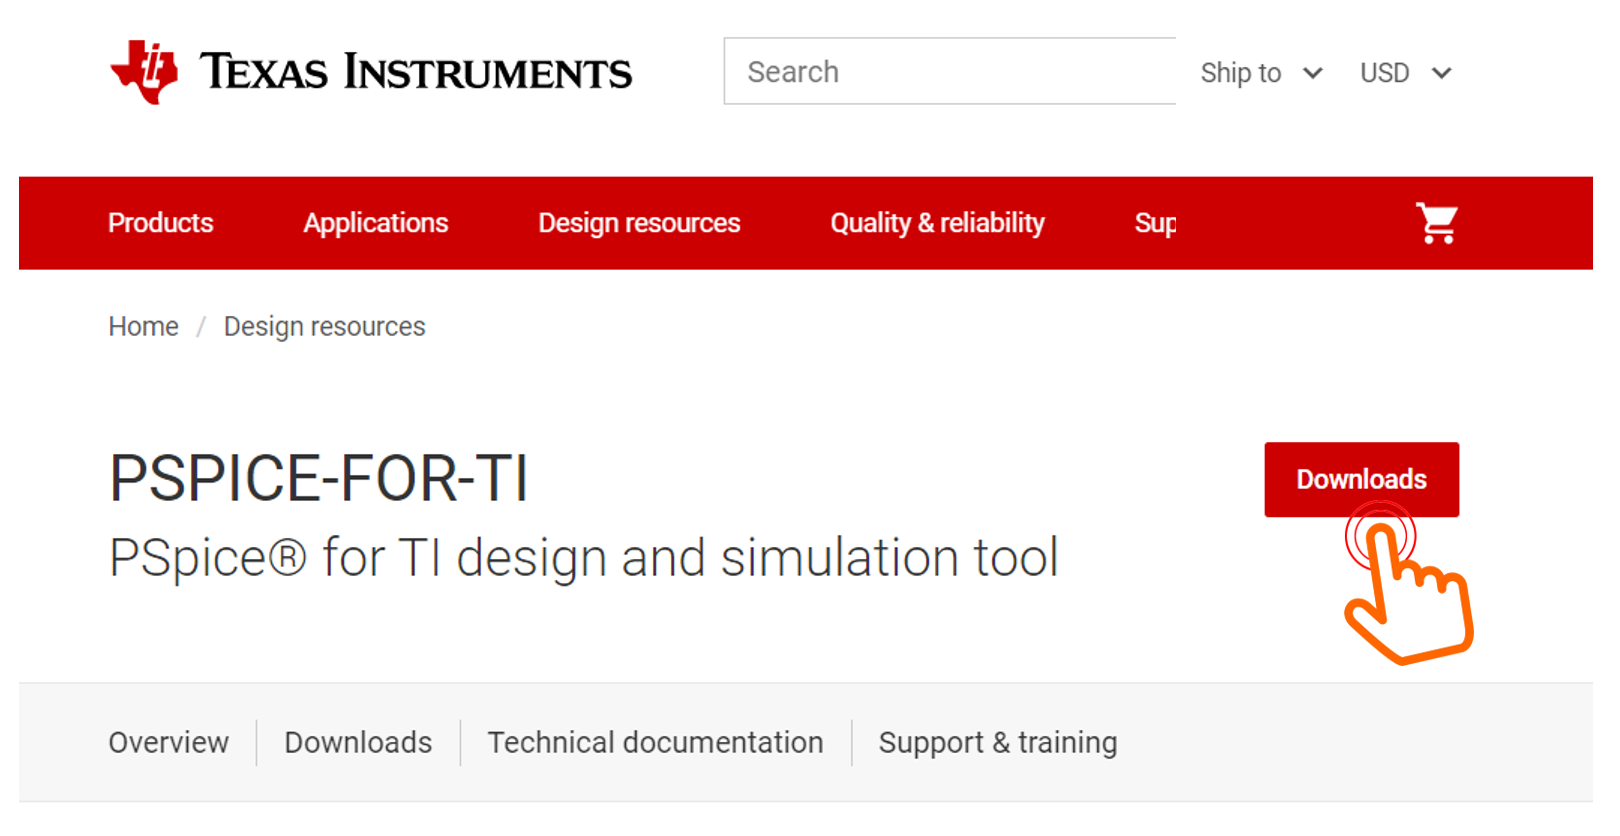
\includegraphics[width=4in]{source/picture/bai_1/pic1.PNG}
    \caption{\textit{Homepage to download PSpice}}
    \label{bai1_pic1}
\end{figure}

By clicking on the \textbf{Download} button, the website is navigated as follows:
\begin{figure}[!htp]
    \centering
    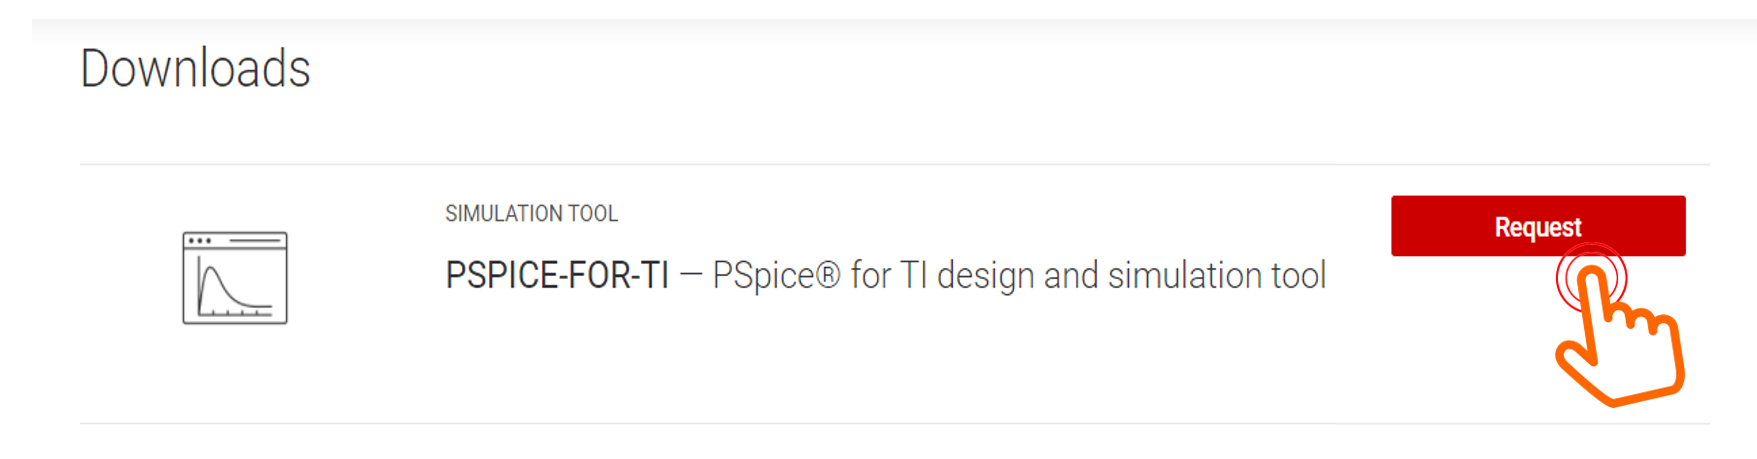
\includegraphics[width=4in]{source/picture/bai_1/pic2.PNG}
    \caption{\textit{Request information for downloading}}
    \label{bai1_pic2}
\end{figure}

Basically, you need to login before requesting a setup file. Please follow the manuals from the website to accomplish this process. An email with an access key will be sent to your account to activate the PSpice software.

\section{Create a project on PSpice}
\textbf{Step 1: } Launch PSpice for TI from windows start menu.
\begin{figure}[!htp]
    \centering
    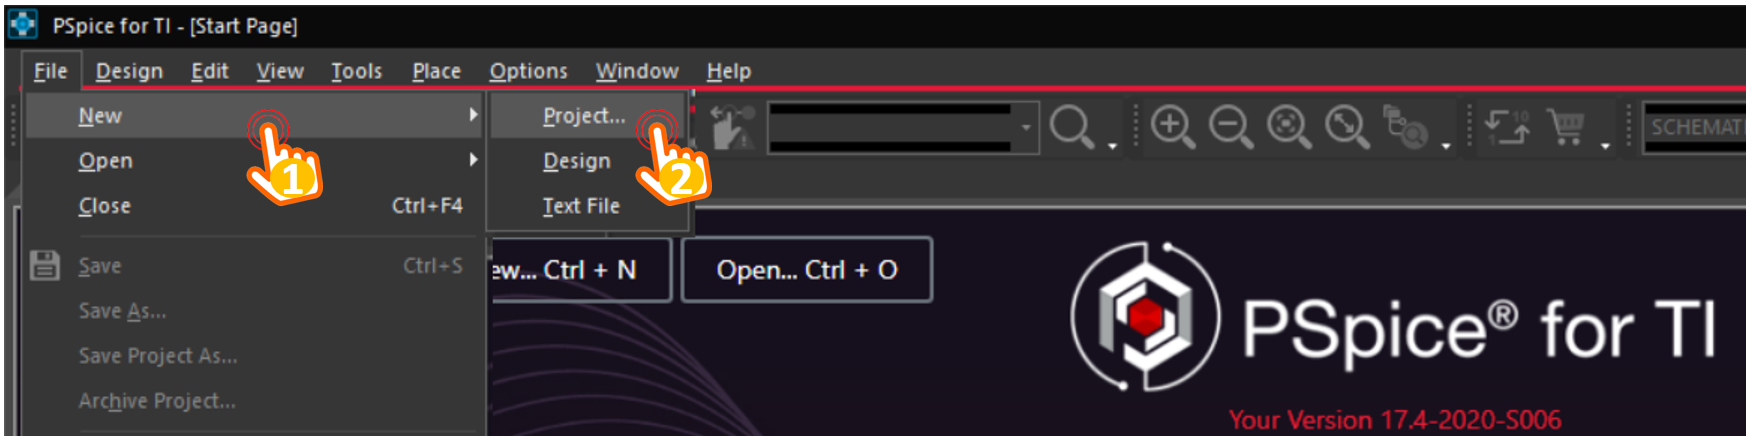
\includegraphics[width=4in]{source/picture/bai_1/pic4.PNG}
    \caption{\textit{Create a new project on PSpice}}
    \label{bai1_pic4}
\end{figure}

From menu \textbf{File}, select \textbf{New}, then select \textbf{Project}.

\textbf{Step 2: } Create an empty project as follows.
\newpage
\begin{figure}[!htp]
    \centering
    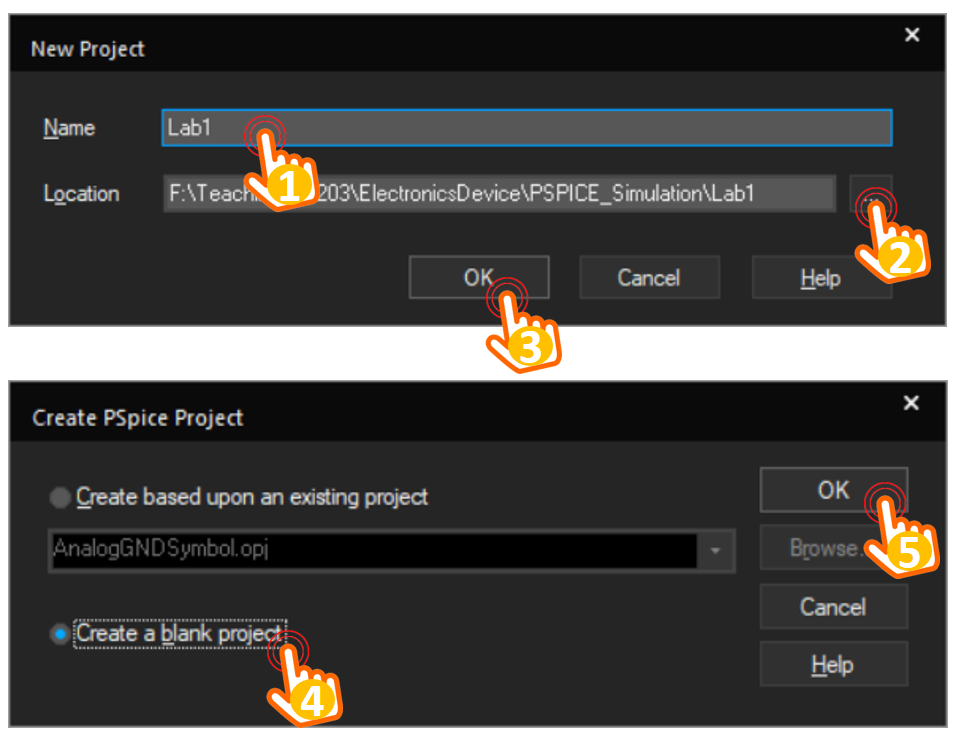
\includegraphics[width=4in]{source/picture/bai_1/pic5.PNG}
    \caption{\textit{Provide the name, location and select a blank project}}
    \label{bai1_pic5}
\end{figure}

In the second dialog, please select \textbf{Create a blank project}. An empty project is created and the next UI is displayed as follow.
\begin{figure}[!htp]
    \centering
    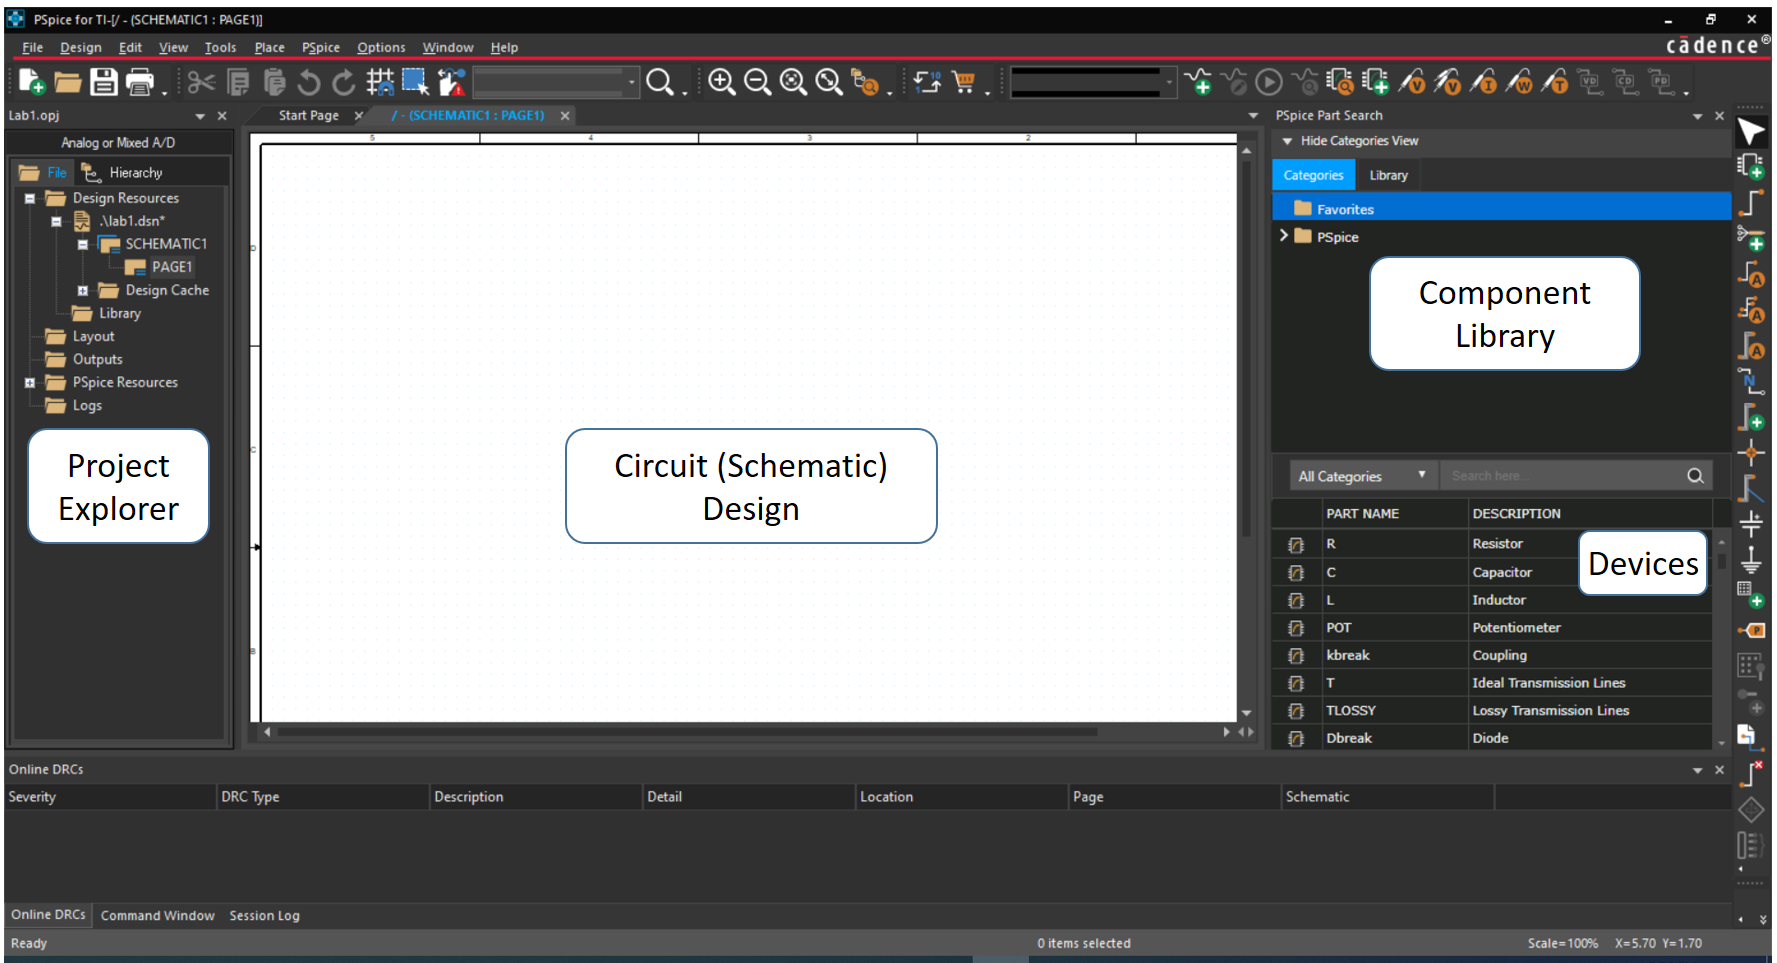
\includegraphics[width=5.5in]{source/picture/bai_1/pic3.PNG}
    \caption{\textit{An empty project is created on PSpice}}
    \label{bai1_pic3}
\end{figure}

\section{Design a circuit}

\textbf{Step 1: } Double click on the Resistor in the device list and then move the mouse to the schematic design page. This device is in the \textbf{Favourite} library in default. While moving, \textbf{press R} to rotate the device before placing it (by left-mouse click), as follow:

\begin{figure}[!htp]
    \centering
    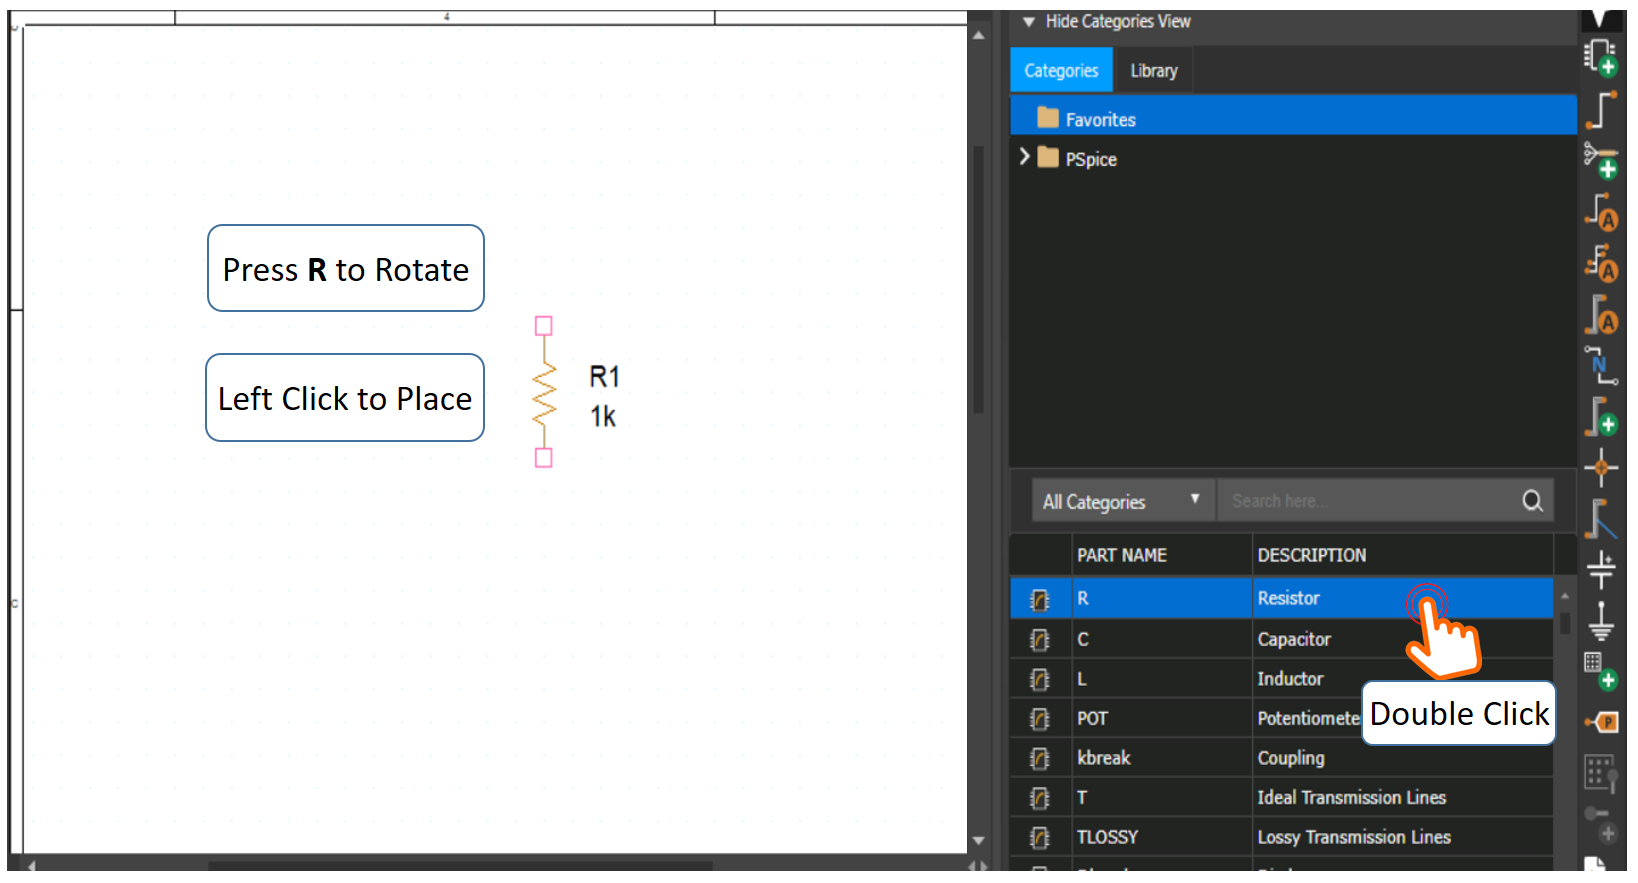
\includegraphics[width=4in]{source/picture/bai_1/pic6.PNG}
    \caption{\textit{Place a resistor in PSpice}}
    \label{bai1_pic6}
\end{figure}

\newpage
\textbf{Step 2: } Double click on the value of the resistor, which is 1k in default, in order to change its resistance.

\begin{figure}[!htp]
    \centering
    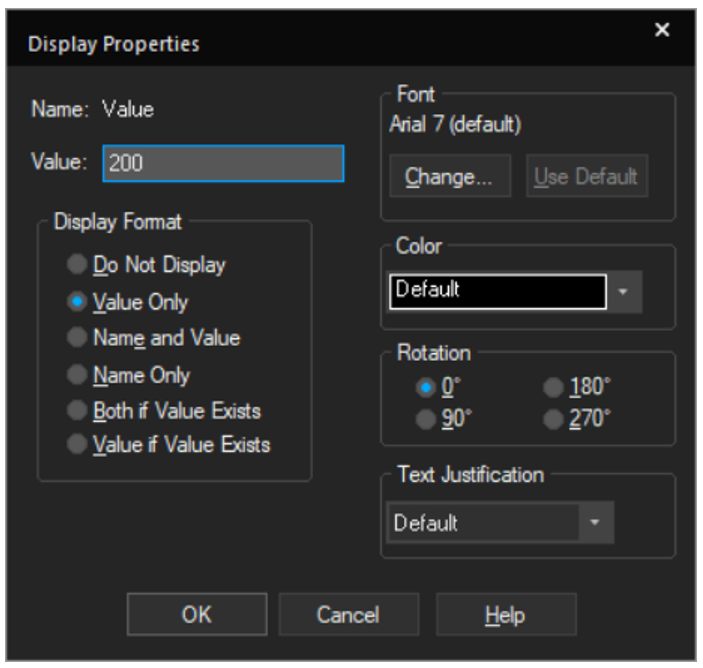
\includegraphics[width=3in]{source/picture/bai_1/pic7.PNG}
    \caption{\textit{Assign the resistance}}
    \label{bai1_pic7}
\end{figure}

If the resistance is Ohm, no unit is required in the \textbf{Value} field. Repeat the first 2 steps to finalize all resistors in the circuit.

\begin{figure}[!htp]
    \centering
    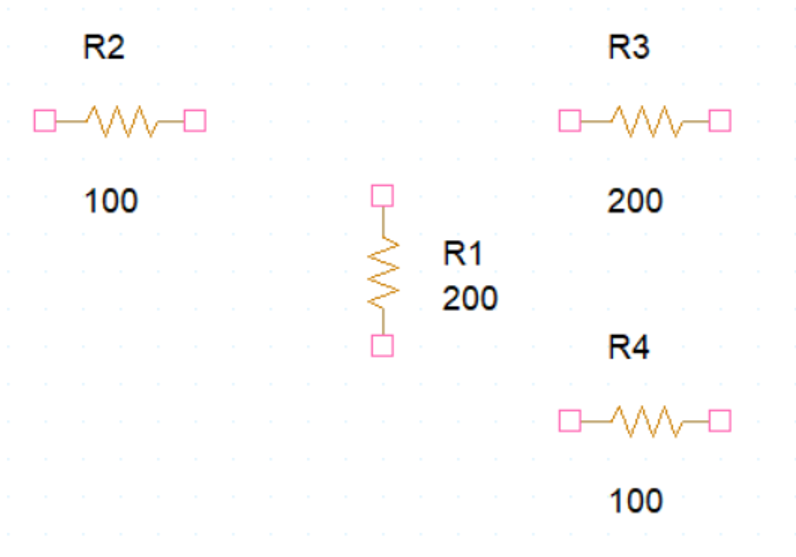
\includegraphics[width=3in]{source/picture/bai_1/pic8.PNG}
    \caption{\textit{Place other resistors in PSpice}}
    \label{bai1_pic8}
\end{figure}

Some hot keys including \textbf{Ctrl + C} and \textbf{Ctrl + V} can be used to copy an old device.\\

\textbf{Step 3: } In order to place a voltage supple, find the component named \textbf{VDC} (DC Voltage Source) in the favourite list, or filter it on the search area. Double click on the voltage supply and change to a desired value. The result after this step is expected as figure bellow.

\begin{figure}[!htp]
    \centering
    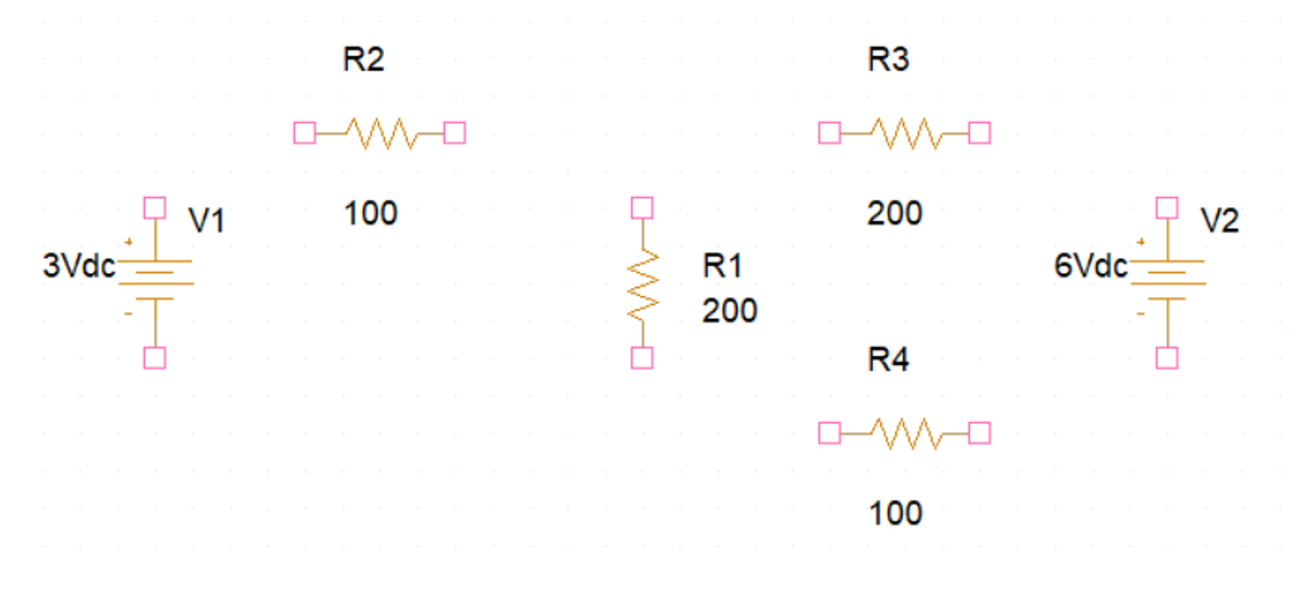
\includegraphics[width=4in]{source/picture/bai_1/pic9.PNG}
    \caption{\textit{Place the power supply using VDC component}}
    \label{bai1_pic9}
\end{figure}

\textbf{Step 4: } Wire all components by selecting the Wire command on the right panel (hot key is W).

\begin{figure}[!htp]
    \centering
    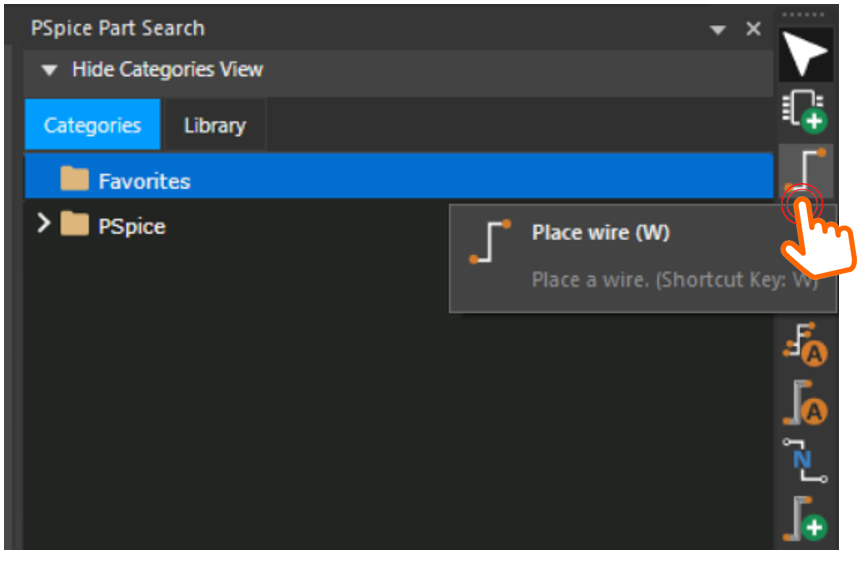
\includegraphics[width=4in]{source/picture/bai_1/pic10.PNG}
    \caption{\textit{Wire the whole circuit}}
    \label{bai1_pic10}
\end{figure}

By clicking a start point and an end point, a wire is placed. In order to delete, select the wire and press \textbf{Delete}. The picture of the circuit after this step is depicted as follow.
\newpage
\begin{figure}[!htp]
    \centering
    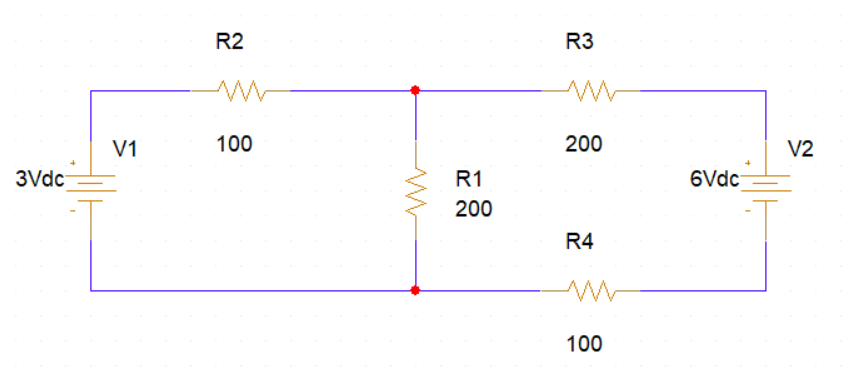
\includegraphics[width=4in]{source/picture/bai_1/pic12.PNG}
    \caption{\textit{Finish all wire in the circuit}}
    \label{bai1_pic12}
\end{figure}

\textbf{Step 5: } Place a Ground symbol. This step is very important to analyze the voltage in a circuit as a reference voltage (0V) is required. The ground symbol is available on the right panel of the software.
\begin{figure}[!htp]
    \centering
    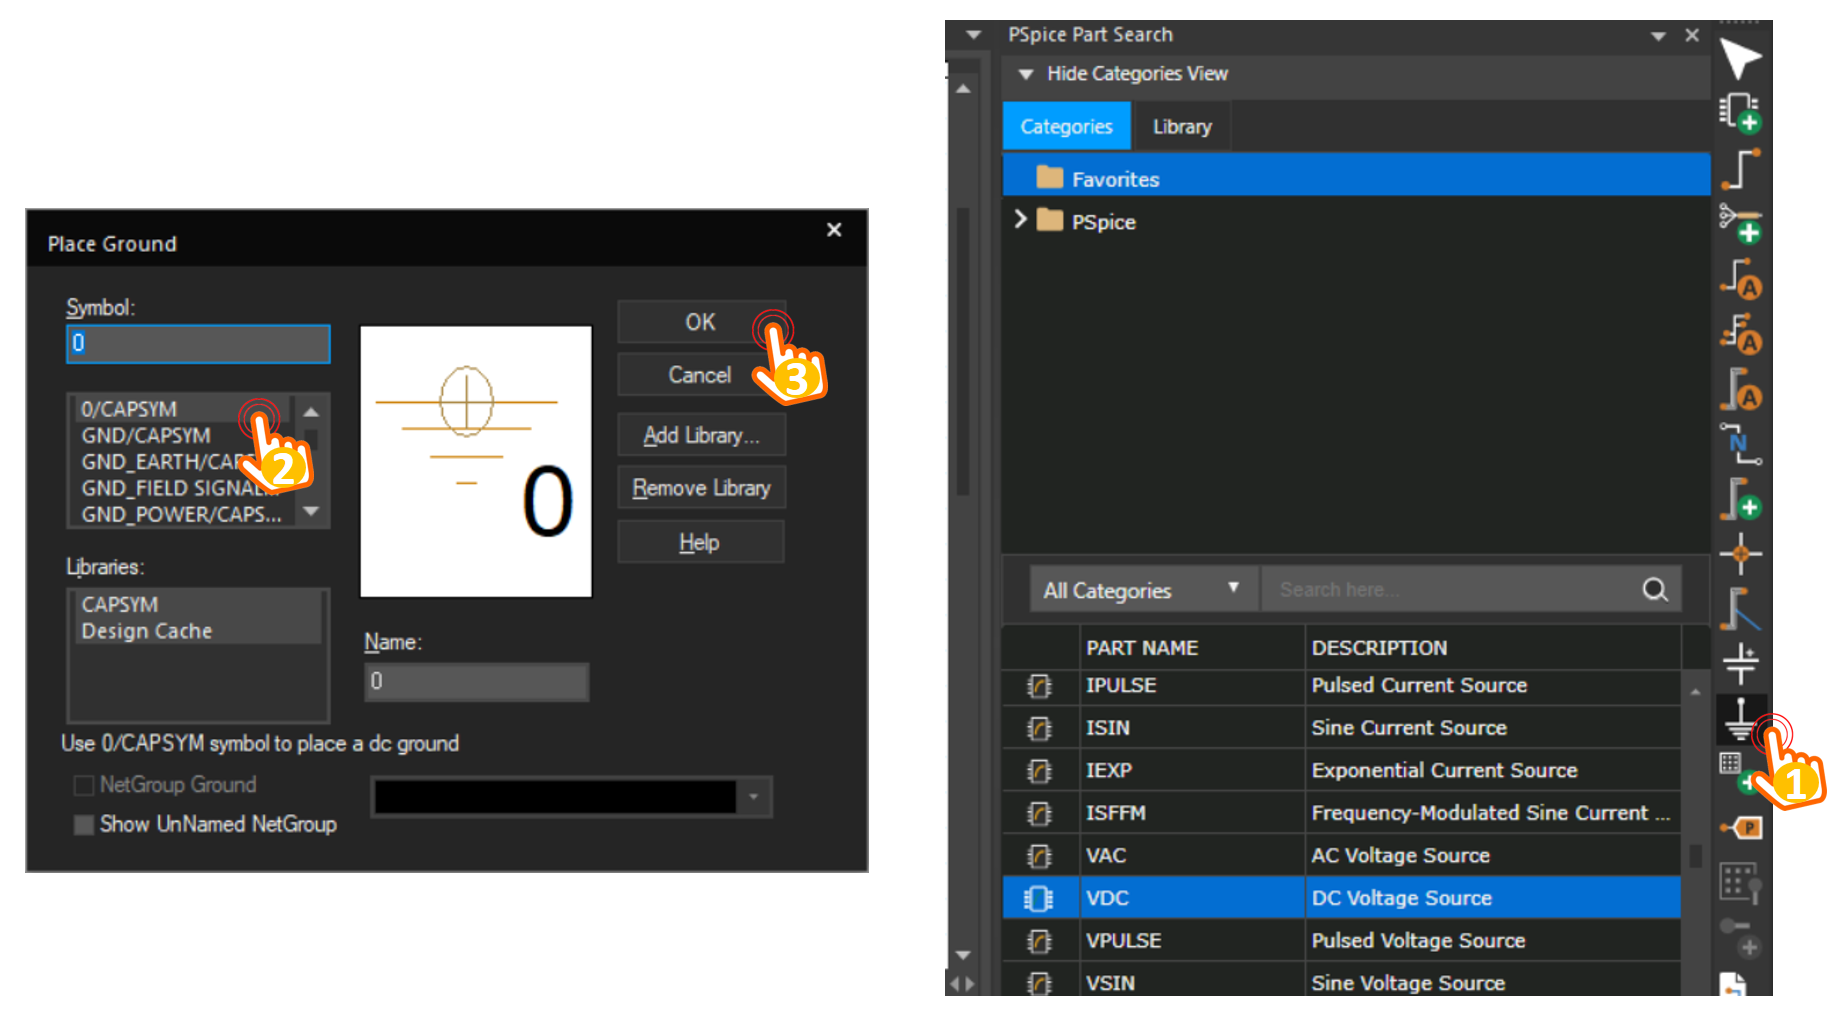
\includegraphics[width=5in]{source/picture/bai_1/pic11.PNG}
    \caption{\textit{Add a ground symbol to the circuit}}
    \label{bai1_pic11}
\end{figure}

Wiring the ground to a point in the circuit, the final result should be like the figure bellow.

\begin{figure}[!htp]
    \centering
    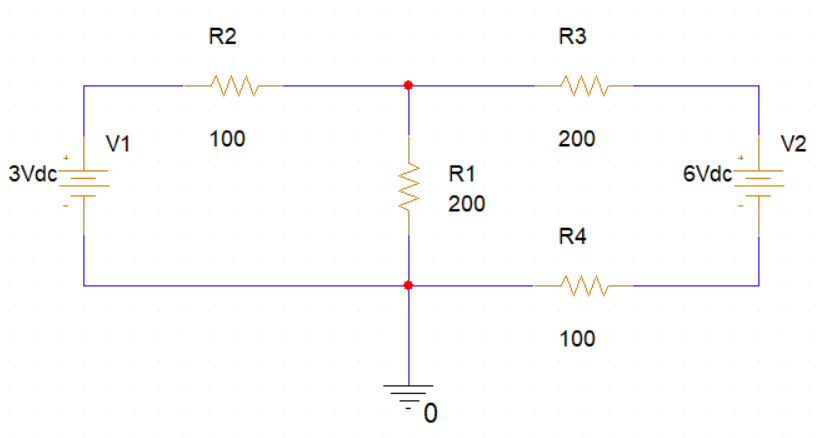
\includegraphics[width=4in]{source/picture/bai_1/pic13.PNG}
    \caption{\textit{A ground point is added to the circuit}}
    \label{bai1_pic13}
\end{figure}

\section{Create a simulation profile}
Before the simulation is started, a simulation profile (or the simulation configuration) is required. From menu \textbf{PSpice}, select \textbf{New Simulation Profile} as follow:
\begin{figure}[!htp]
    \centering
    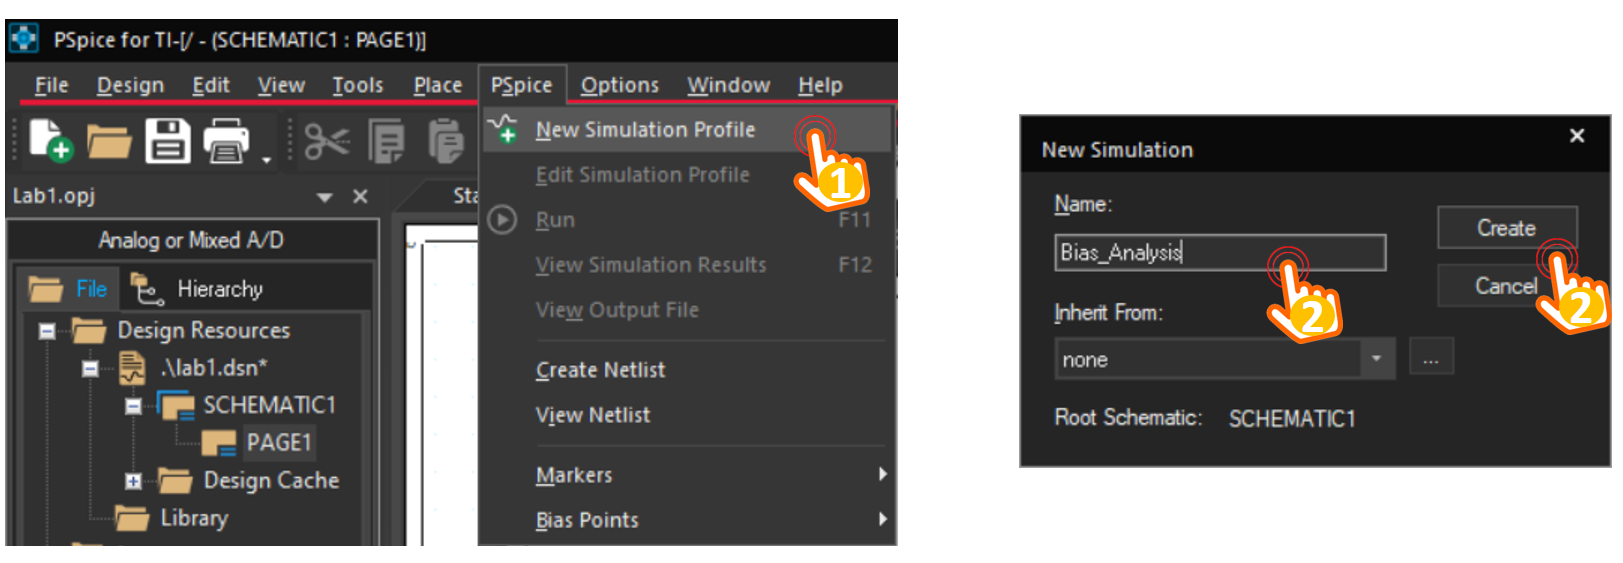
\includegraphics[width=5.5in]{source/picture/bai_1/pic14.PNG}
    \caption{\textit{Create a simulation profile}}
    \label{bai1_pic14}
\end{figure}

When the simulation setting dialog is appeared, please select the \textbf{Bias Point} for analysis type.
\begin{figure}[!htp]
    \centering
    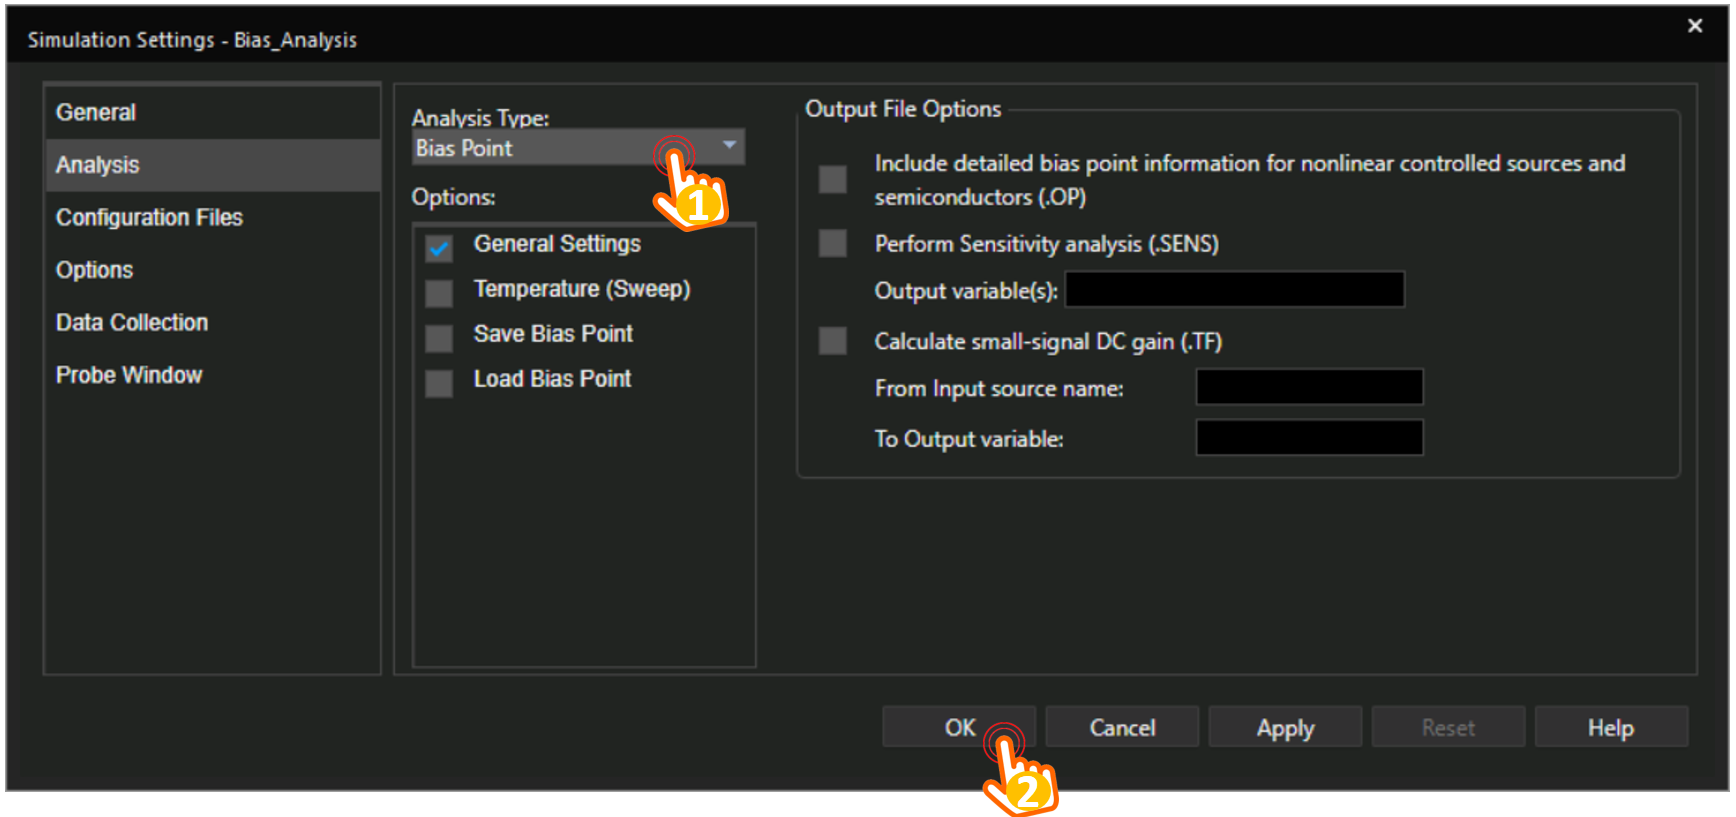
\includegraphics[width=4in]{source/picture/bai_1/pic15.PNG}
    \caption{\textit{Select Bias Point simulation}}
    \label{bai1_pic15}
\end{figure}

In PSpice, the bias point analysis calculates the node voltages and currents through the devices in the circuit. Bias point analysis also takes into account any voltage sources applied to the circuit and any initial conditions set on devices or nodes in the circuit. \\

Finally, click on menu \textbf{PSpice} to select \textbf{Run}, or press \textbf{F11} to start the simulation. The simulation results are displayed directly on the circuit as follow:

\begin{figure}[!htp]
    \centering
    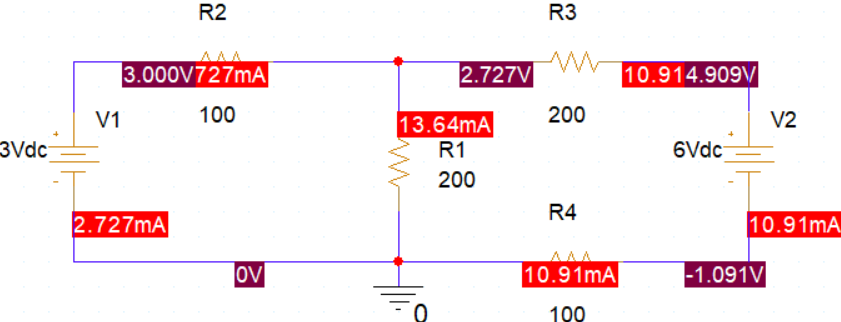
\includegraphics[width=4in]{source/picture/bai_1/pic16.PNG}
    \caption{\textit{Volate and Current in the whole circuit}}
    \label{bai1_pic16}
\end{figure}

In order to display simulation results, go to menu \textbf{PSpice}, select \textbf{Bias Point} and enable the information you need. Students are also proposed to double check their solutions with the simulation results.

\def\answer{1}
\section{Exercise and Report}
In this section, students are proposed to work in some circuit analysis, mostly based on resistors. Some explanations are required and will be considered as a part of the report. Note that the calculation subsection expects to see formulas and equations rather than only the results.

\subsection{Exercise 1}
Given the following circuit. Calculate the value of the voltage $v_0$ and the current $i$. Then, simulate the circuit to check it out.

\begin{figure}[!htp]
    \centering
    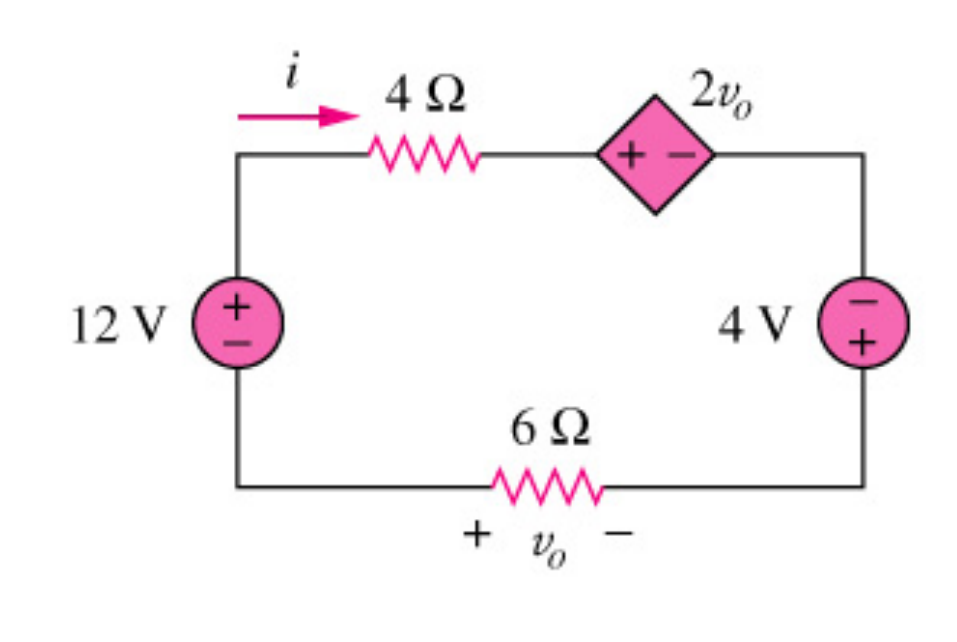
\includegraphics[width = 7cm]{source/picture/bai_1/Bai1_de.png}
    \caption{Find the voltage and the current in the given circuit using KVL}
    \label{lab1_ex1_de}
\end{figure}

\subsubsection{Calculation}
\textit{\textbf{Notes:}}\\
\textit{Explanations, formulas, and equations are expected rather than only results.}\\

According to the:  Kirchoff Voltage Law (KVL)\bigskip\\
We have the first equation:  \dotfill $-4i+2v_0-4-v_0-12=0$ \dotfill\bigskip(1)\\
According to the:  Ohm's Law\bigskip\\
We have the second equation: \dotfill $v_0 = 6i$\dotfill\bigskip(2)\\
From (1) and (2) we have:\bigskip\\
$v_0 = 48$ \dotfill\bigskip\\
$i = 8$ \dotfill\bigskip\\

\subsubsection{Simulation}

\textbf{\textit{Tips:}}\\
To get the Voltage Controlled Voltage Source (VCVS) from the PSpice, under the \textit{\textbf{Place}} menu, find \textbf{\textit{PSpice Component > Source > Controlled Sources > VCVS}}.

A circuit used for the simulation in this exercise maybe like this:
\begin{figure}[H]
    \centering
    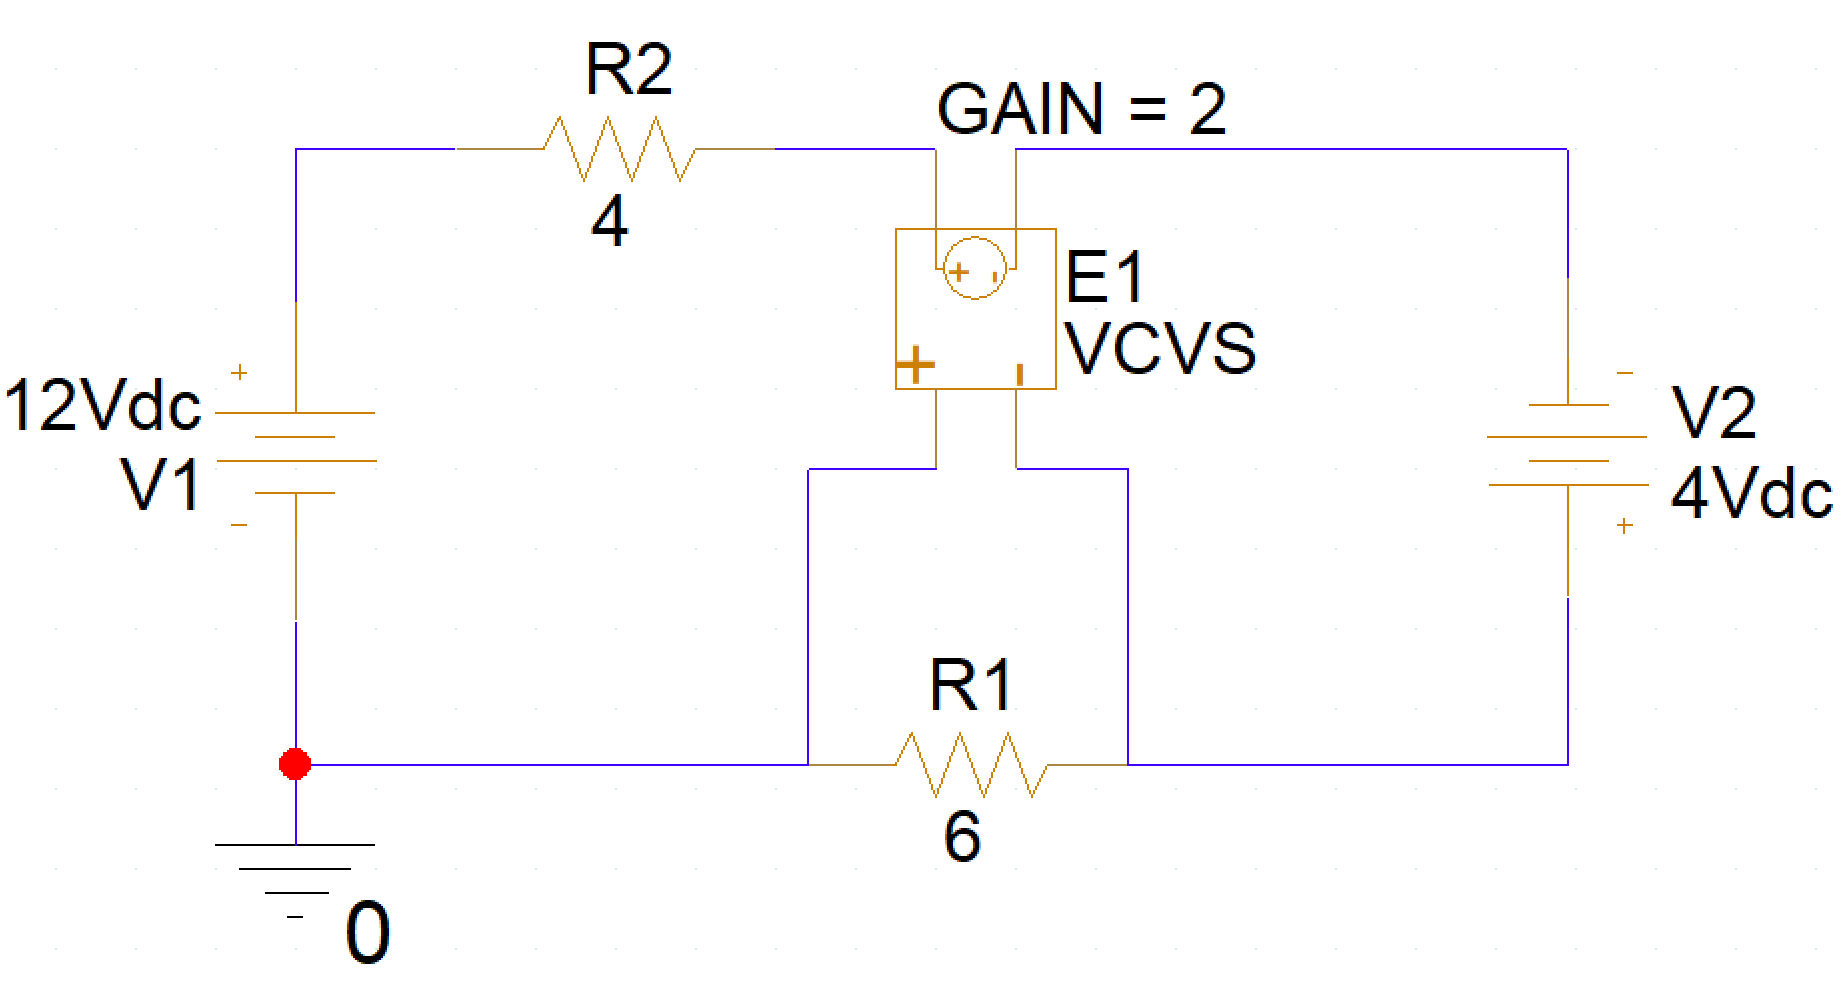
\includegraphics[width = 10cm]{source/picture/bai_1/Bai1_ps.png}
    \caption{A circuit containing a Voltage Controlled Voltage Source in PSpice}
\end{figure}

\textit{\textbf{Simulation result (image):}}
\begin{figure}[H]
    \centering
    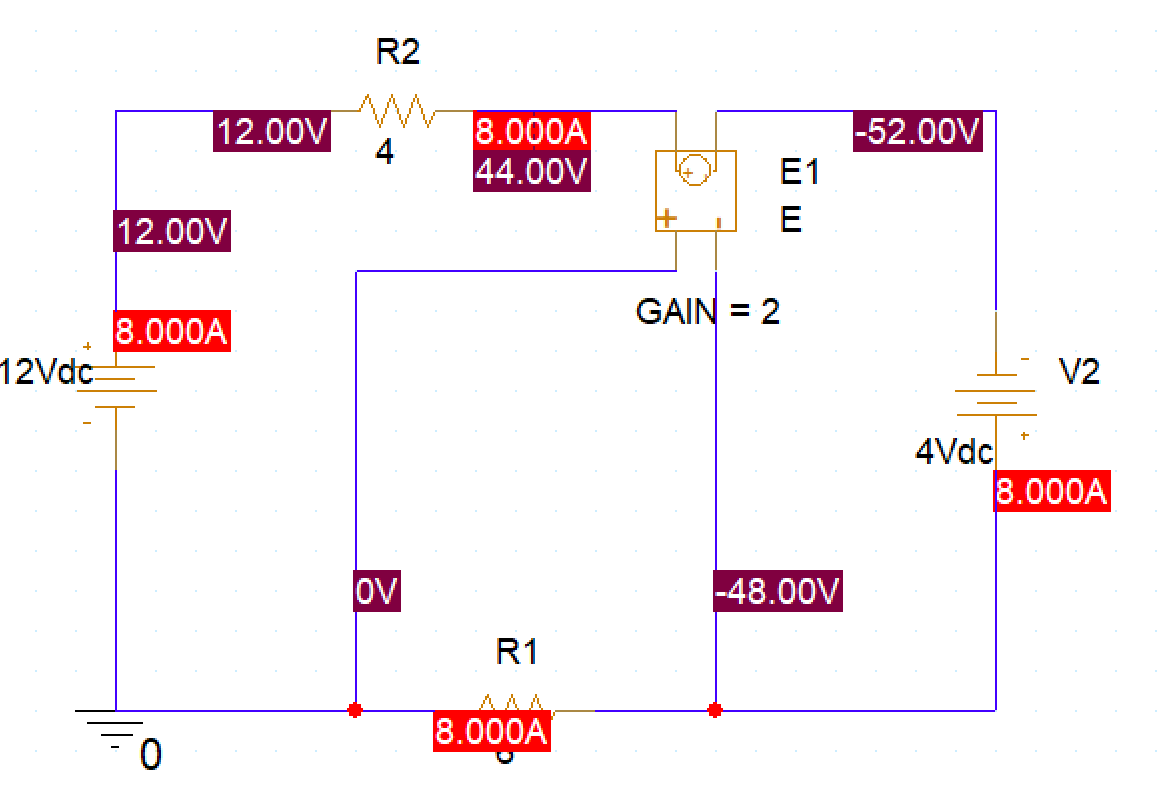
\includegraphics[width = 10cm]{source/picture/bai_1/ex1.png}
\end{figure}
\newpage

\subsection{Exercise 2}
Given the following circuit, students rearrange the circuit to clarify its serial and/or parallel topology. Then, apply the knowledge you've learned to find the equivalent resistance value between two circuit terminals A and F. Finally, perform the simulation to check if the current through the whole circuit is correctly calculated.

\begin{figure}[H]
    \centering
    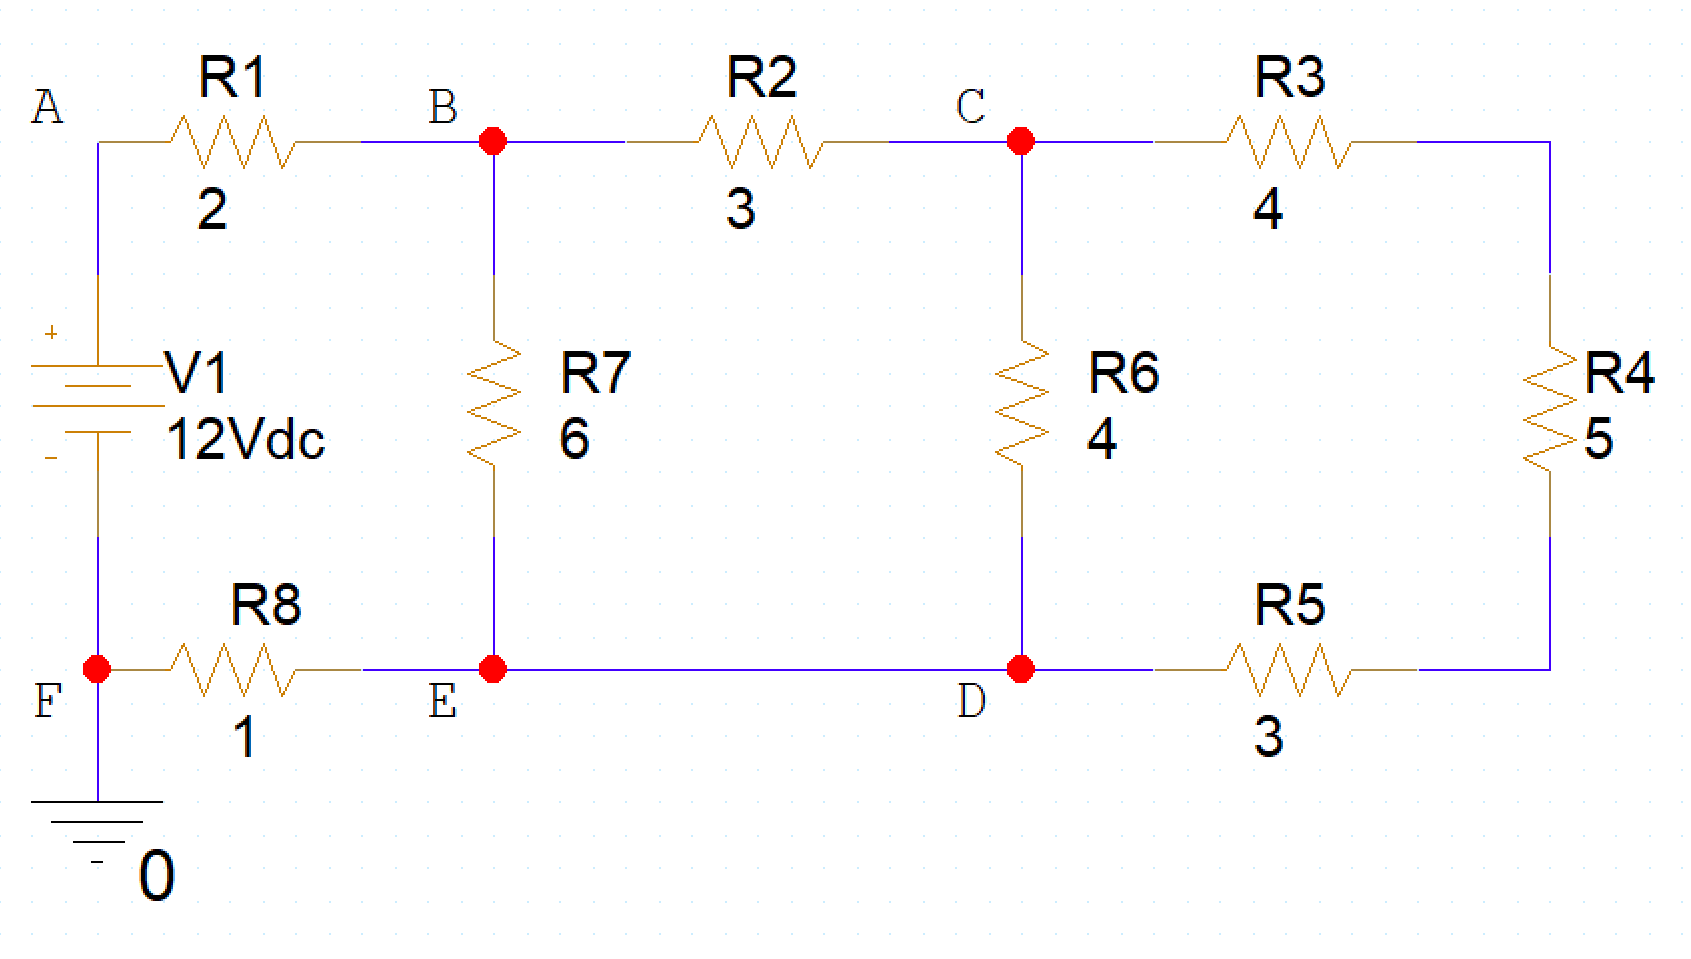
\includegraphics[width = 10cm]{source/picture/bai_1/Bai2_de.png}
    \caption{Find the equivalent resistance value between terminals A and F}
    \label{lab1_ex2_de}
\end{figure}

\subsubsection{Rearrange the circuit}
\textit{Insert the rearranged circuit here. Don't forget the resistance values and the nodes' names.}
\begin{figure}[H]
    \centering
    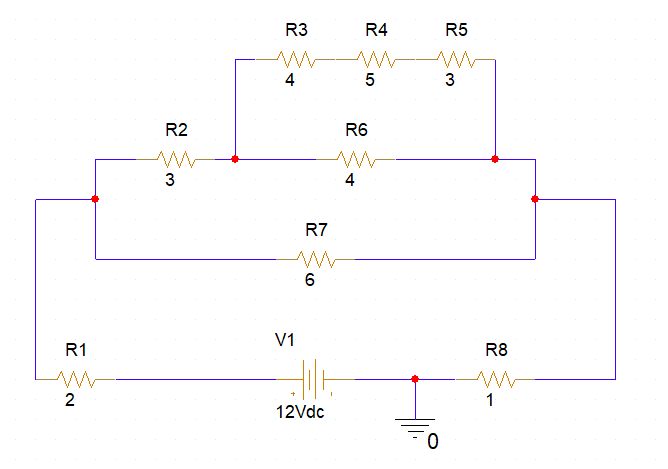
\includegraphics[width = 10cm]{source/picture/bai_1/ex2.png}
    \label{lab1_ex2}
\end{figure}
\newpage

\subsubsection{Calculation}
\textit{\textbf{Convention:}}\\
\textit{The equivalent resistance between the two terminals A and B of a circuit segment containing only R1, R2, R3, and R4 may be named $R_{AB\_1234}$.}\\
\\
\textit{\textbf{Notes:}}\\
\textit{Explanations, formulas, and equations are expected rather than only results.}\\
\\
$R_{CD\_3456} = \frac{R_6(R_3+R_4+R_5)}{R_3+R_4+R_5+R_6}=3\Omega$  as $R_6$ // $R_{345}$\bigskip\\
$R_{BE} = (\frac{1}{R_{CD}+R_2}+\frac{1}{R_7})^{-1}= \frac{1}{6} +\frac{1}{3+3}=3\Omega$ as $R_{CD},R_2$ // $R_7$\bigskip\\
$R_{AF} = R_{BE} + R_1 + R_8 = 3+2+1=6\Omega$\bigskip\\
$I_{AB} = I = \frac{U}{R_{eq}} = \frac{U}{R_{AF}} = \frac{12}{6} = 2A$ Ohm's Law\bigskip\\

\subsubsection{Simulation}
\textit{\textbf{Simulation result (image):}}
\begin{figure}[H]
    \centering
    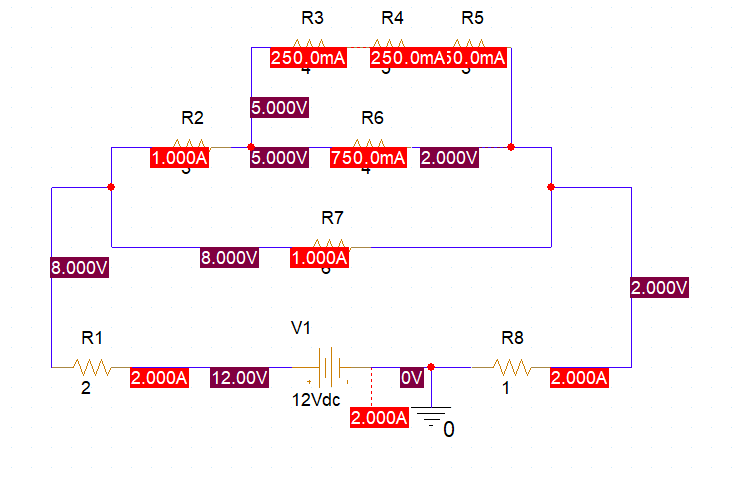
\includegraphics[width = 10cm]{source/picture/bai_1/ex2_sim.png}
\end{figure}
\newpage

\subsection{Exercise 3}
Given the following circuit, students rearrange the circuit to clarify its serial and/or parallel topology. Next, apply the knowledge you've learned to find the equivalent resistance value between two circuit terminals A and F, the voltage values at A, B, C, D, and E. Finally, perform the simulation to check your calculation.

\begin{figure}[H]
    \centering
    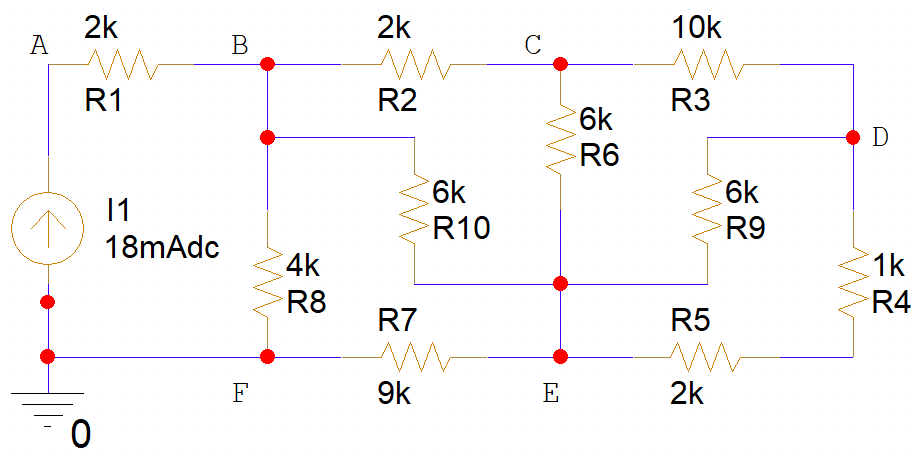
\includegraphics[width = 11cm]{source/picture/bai_1/LAB1_EX3_de.png}
    \caption{Find the whole-circuit equivalent resistance and the voltages at A, B, C, D, and E}
    \label{lab1_ex3_de}
\end{figure}

\subsubsection{Rearrange the circuit}
\textit{Insert the rearranged circuit here. Don't forget the resistance values and the nodes' names.}
\begin{figure}[H]
    \centering
    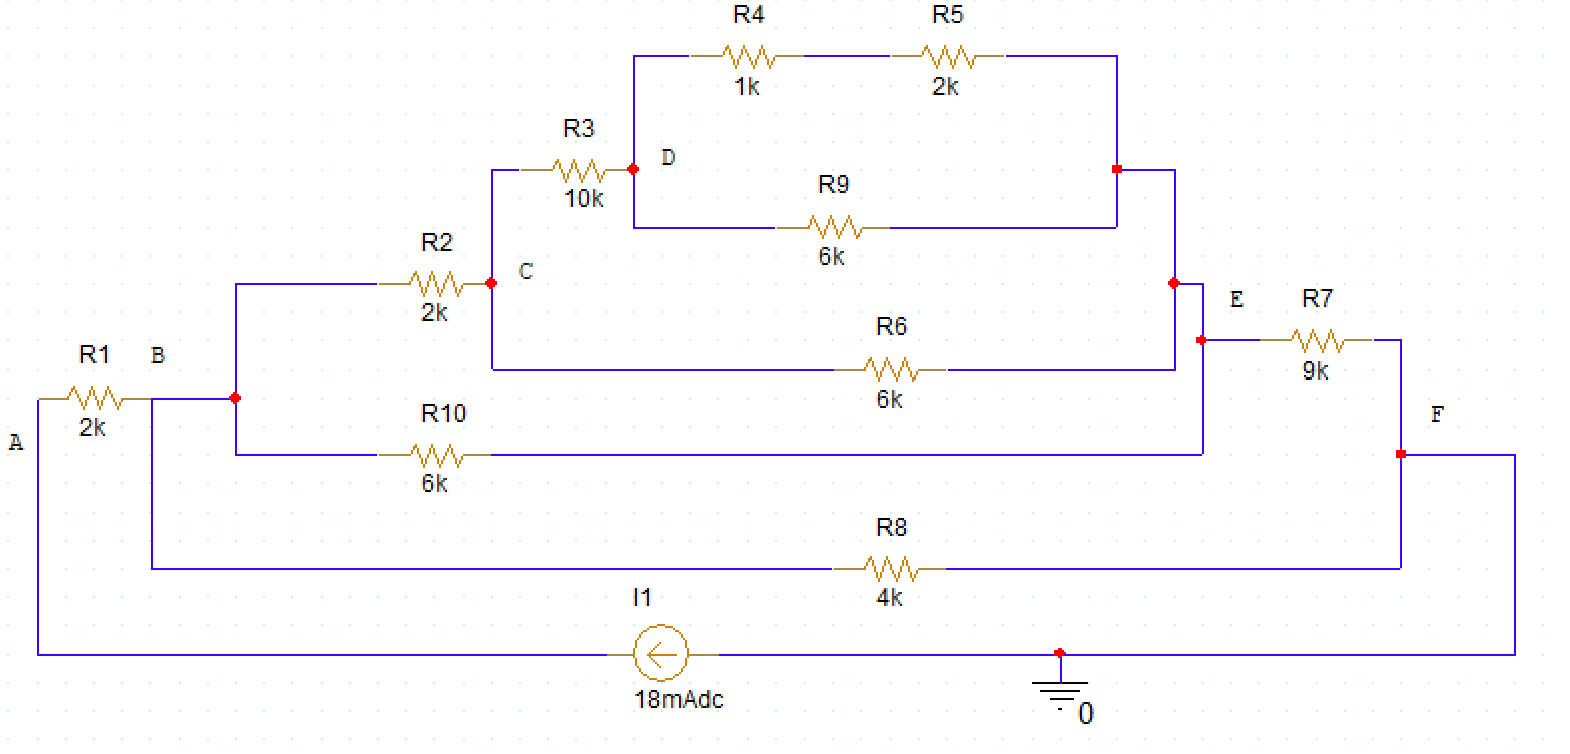
\includegraphics[width = 10cm]{source/picture/bai_1/ex3_rearrange.png}
\end{figure}
\newpage

\subsubsection{Calculation}
\textit{\textbf{Notes:}}\\
\textit{Explanations, formulas, and equations are expected rather than only results.}\\
\\
$$R_{CE} = \left(\frac{1}{R_6}+\frac{1}{R_3 + \frac{R_9(R_4+R_5)}{R_9+R_4+R_5}}\right)^{-1} = \left(\frac{1}{6}+\frac{1}{10 + \frac{6(1+2)}{6+1+2}}\right)^{-1} = 4(k\Omega)$$
$$R_{BE} = \left(\frac{1}{R_10} + \frac{1}{R_2 + R_{CE}}\right)^{-1} = \left(\frac{1}{6}+\frac{1}{2+4}\right)^{-1} = 3(k\Omega)$$
$R_{AF} =R_1 + \frac{R_8(R_{BE}+R_7)}{R_8 + R_{BE} + R_7} = 2 + \frac{4(3+9)}{4+3+9} = 5(k\Omega)$ \bigskip\\
$V_A = I_1 \times R_{AF} = 18 \times 5 = 90 $ \bigskip\\
$V_B = V_A - R_1 \times I_1 = 90 -2 \times 18 = 54$ \bigskip\\
$V_C = V_B - \left(\frac{V_B-V_E}{R_{BE}} - \frac{V_B-V_E}{R_{10}}\right) \times R_2 = 54 - \left(\frac{54-40.5}{3} - \frac{54-40.5}{6}\right) \times 2 = 49.5 (V)$ \bigskip\\
$V_D = V_C - \left(\frac{V_C-V_E}{R_{CE}} - \frac{V_C-V_E}{R_{6}}\right) \times R_3 = 49.5 - \left(\frac{49.5-40.5}{4} - \frac{49.5-40.5}{6}\right) \times  10= 42 (V)$ \bigskip\\
$V_E = V_F + \left(\frac{V_A}{R_{BF}} - \frac{V_A}{R_8}\right) \times 9 = 0 + \left(\frac{54}{3} - \frac{54}{4}\right) \times 9 = 40.5 (V)$ \bigskip\\

\subsubsection{Simulation}
\textit{\textbf{Simulation result (image):}}
\begin{figure}[H]
    \centering
    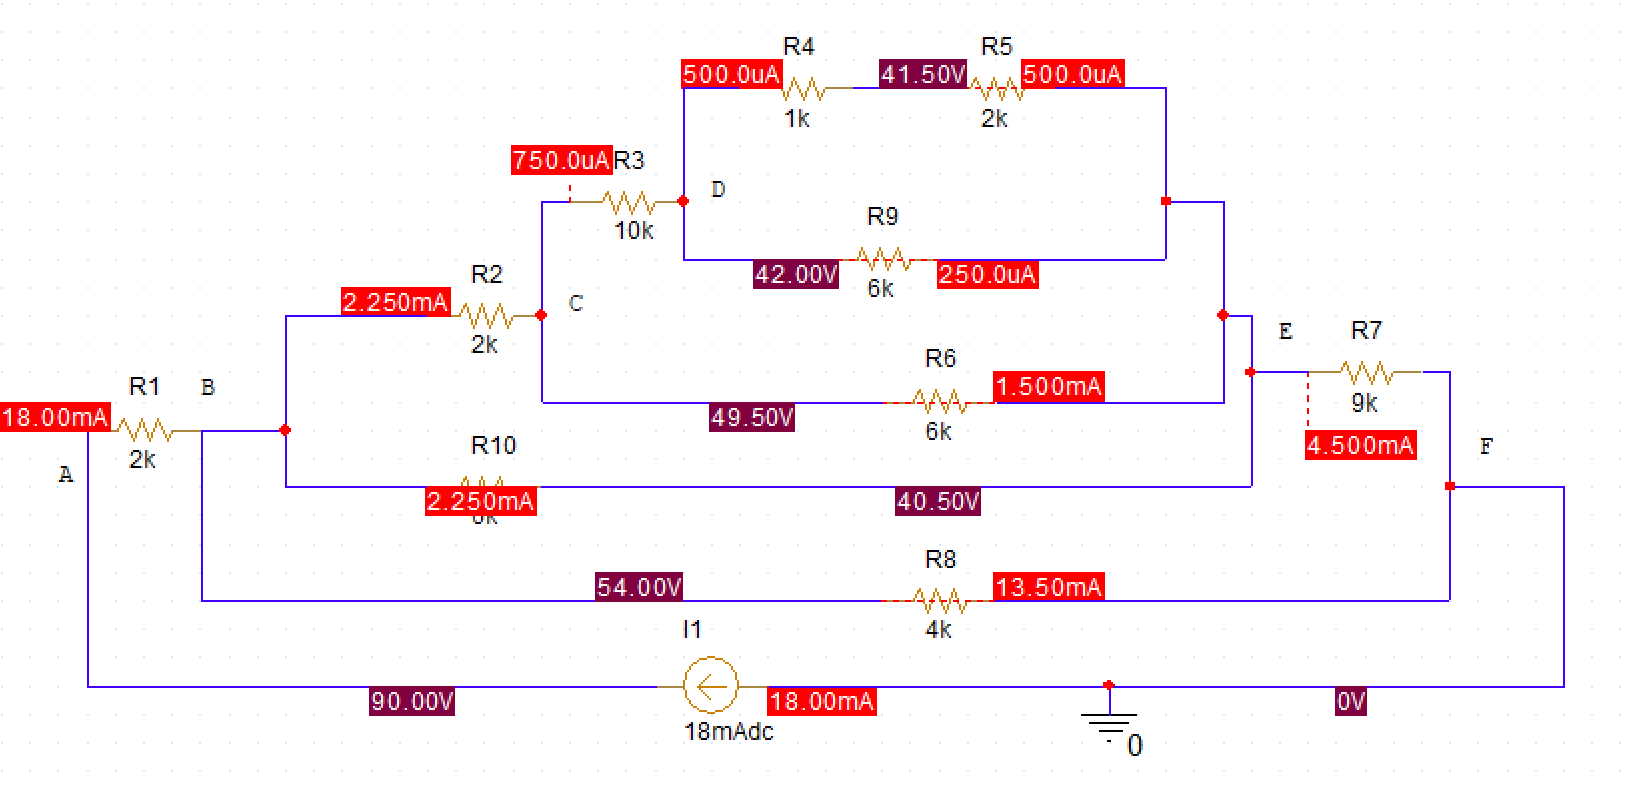
\includegraphics[width = 10cm]{source/picture/bai_1/ex3_sim.png}
\end{figure}
\newpage

\subsection{Exercise 4}
Given the following circuit, find $I_1$, $I_2$, $I_3$, $V_a$, and $V_b$. Present your calculation steps and check them out by performing the simulation.

\begin{figure}[H]
    \centering
    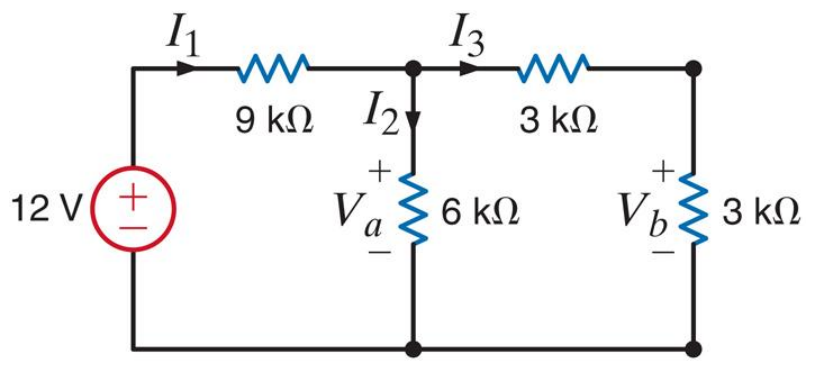
\includegraphics[width = 8cm]{source/picture/bai_1/lab1_ex4_de.png}
    \caption{Find $I_1$, $I_2$, $I_3$, $V_a$, and $V_b$}
    \label{lab1_ex4_de}
\end{figure}

\subsubsection{Calculation}
\textit{\textbf{Notes:}}\\
\textit{Explanations, formulas, and equations are expected rather than only results.}\\
\\ \\
Equivalent Resistor:
$$ R_{eq} = R_1 + \left(\frac{1}{R_2 + R_3} + \frac{1}{R_4} \right)^{-1} = 9 + \frac{(3+3)6}{3 + 3 + 6} = 12(k\Omega) $$

Using KCL: $I_1 = I_2 + I_3$\\
Using KVL:
$\begin{cases}
        -12 + 9I_1 + 6I_2 = 0 \\
        -6I_2 + 3I_3 + 3I_3 = 0
    \end{cases}$ \\
Solving the system of three aforementioned equations:
$\begin{cases}
        I_1 = 1 (mA)  \\
        I_2 = 0.5(mA) \\
        I_3 = 0.5(mA)
    \end{cases}$
\\
$V_a = 6 \times I_2 = 6 \times 0.5 = 3 (V)$ \\
$V_b = 3 \times I_3 = 3 \times 0.5 = 1.5(V)$ \\


\subsubsection{Simulation}
\textit{\textbf{Simulation result (image):}}
\begin{figure}[H]
    \centering
    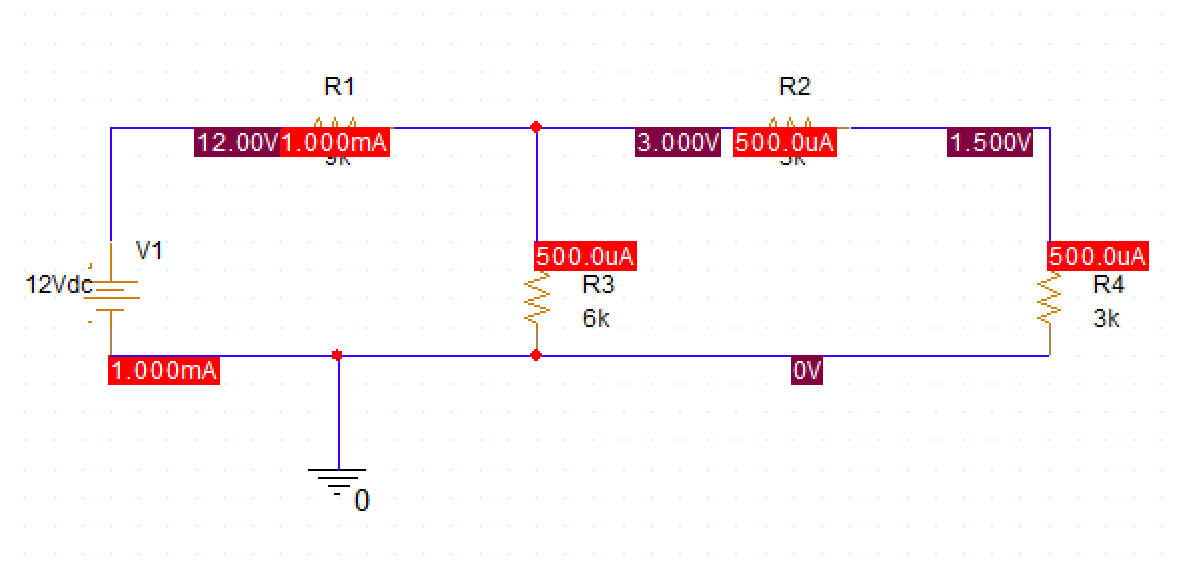
\includegraphics[width = 10cm]{source/picture/bai_1/ex4_sim.png}
\end{figure}
\newpage

\subsection{Exercise 5}
Given the network as shown below:

\begin{figure}[H]
    \centering
    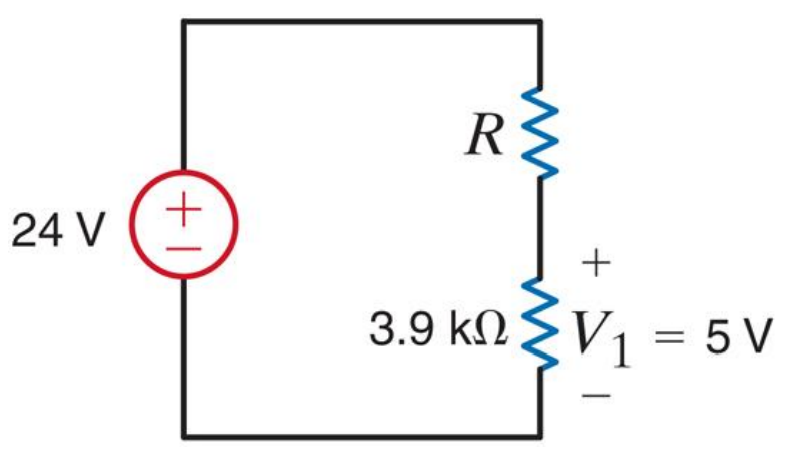
\includegraphics[width = 6cm]{source/picture/bai_1/lab1_ex5_de.png}
    \caption{Select resistor R from the standard resistors list and do the following requirement}
    \label{lab1_ex5_de}
\end{figure}

\textit{\textbf{Notes:}}\\
\textit{Explanations, formulas, and equations are expected rather than only results.}\\

\begin{enumerate}[label=\alph*.]
    \item Find the required value for the resistor R.\bigskip\\
          $R = 14.82 (k\Omega)$ as $3.9 \frac{24}{3.9+x} = 5$\medskip
    \item Use Table 2.1 in the lecture slide to select a standard 10\% tolerance resistor for R. R in the circuit may be a single resistor or a combination of many resistors as long as these resistors are meet the standard values and are available in the market.\bigskip\\
          \\
          The selected resistor: $R = 15 (k\Omega) \pm 10\%$\bigskip
    \item Using the resistor selected in (b), determine the voltage across the 3.9k resistor.\bigskip\\
          The value of $V_1$ according to the selected resistor R:$3.9 \times \frac{24}{3.9 + 15} = 4.9524 (k\Omega)$\medskip
    \item Calculate the percent error in the voltage V1, if the standard resistor selected in (b) is used.\\
          $$\frac{V_{1'}^{2}}{R} = \frac{4,9524^2}{3.9} = 5,28879 $$
    \item Determine the power rating for this standard component.\bigskip\\
          $P_R = RI^2 = 15 \times \left(\frac{24}{3.9+15}\right)^2 = 24.1875 (mW)$\dotfill\
\end{enumerate}

\subsubsection{Simulation}
\textit{\textbf{Simulation result (image):}}
\begin{figure}[H]
    \centering
    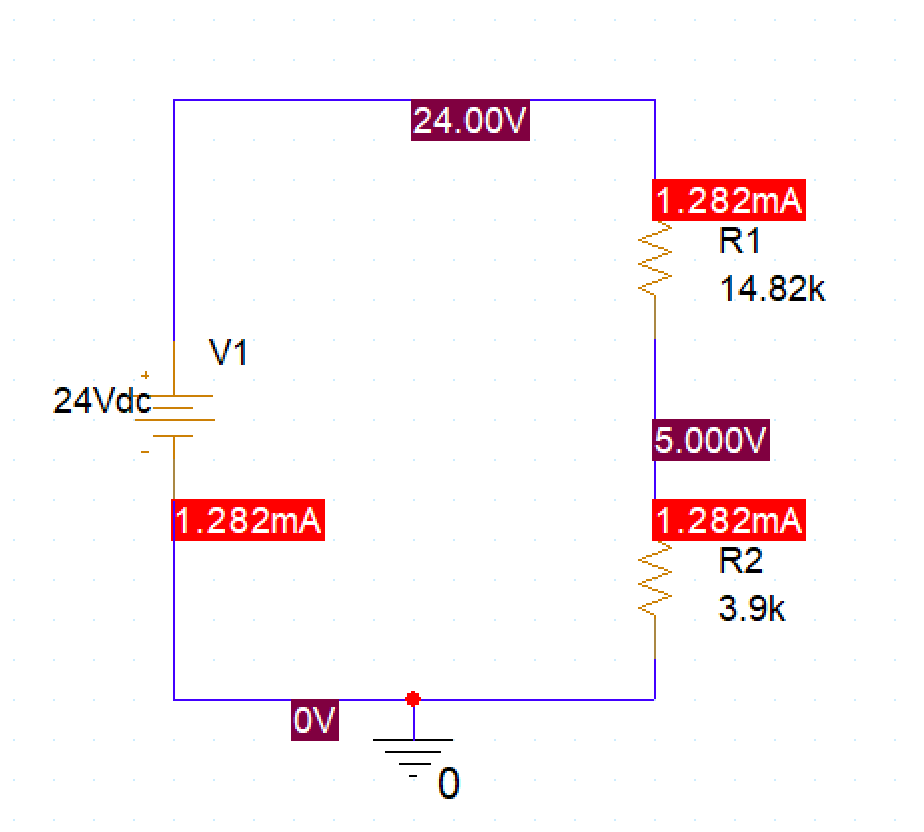
\includegraphics[width = 10cm]{source/picture/bai_1/ex5_sim.png}
\end{figure}

\newpage

\subsection{Exercise 6}
Given the following circuit. Apply the knowledge you've learned to transform it into another form in which you can find total equivalent resistance $R_{ab}$ more easily. Next, find the value of the current $i$ through the circuit and perform a simulation to check it out.

\begin{figure}[H]
    \centering
    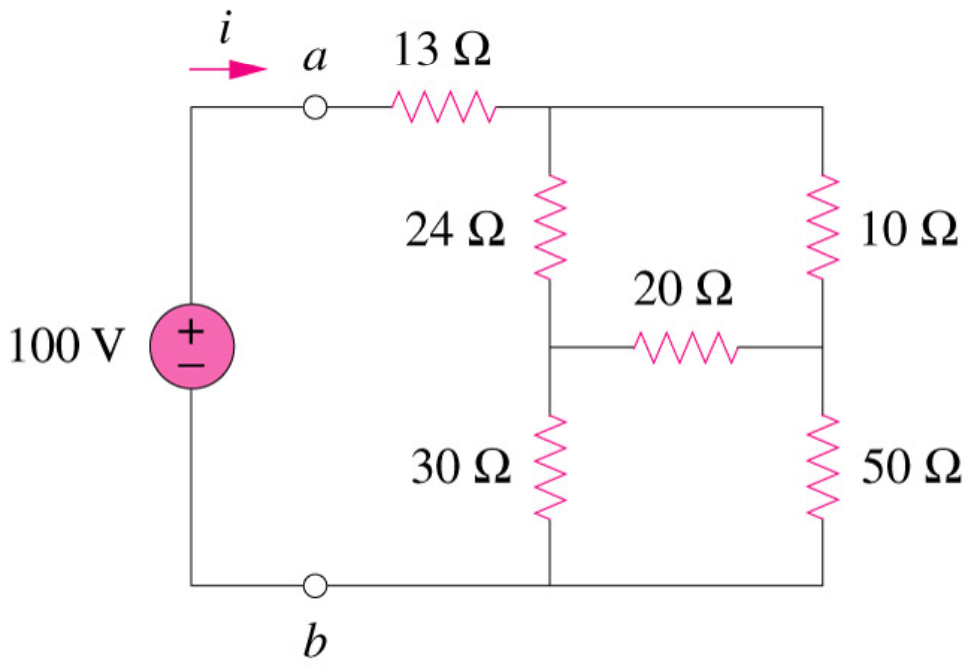
\includegraphics[width = 9cm]{source/picture/bai_1/lab1_ex6_de.png}
    \caption{Transform the circuit, then find the equivalent resistance $R_{ab}$ and the current $i$ through the circuit.}
    \label{lab1_ex6_de}
\end{figure}

\subsubsection{Circuit transformation}
\textit{Insert the transformed circuit here.}
\begin{figure}[H]
    \centering
    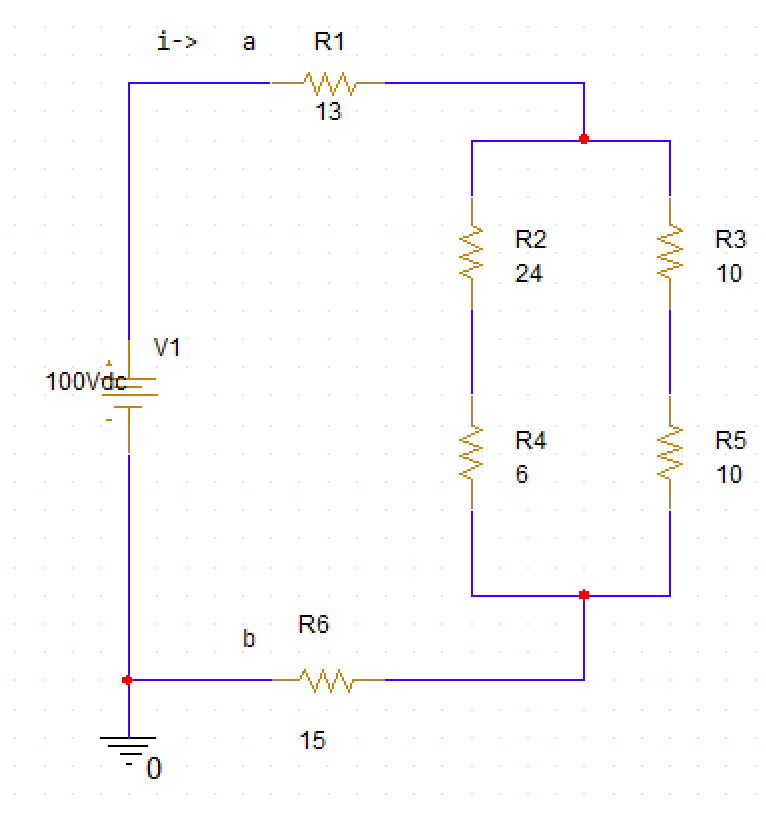
\includegraphics[width = 10cm]{source/picture/bai_1/ex6_rearrange.png}
\end{figure}
\newpage
\textit{Explain any calculations (i.e., write out the formulas you used).}\\
\bigskip
Apply Delta - Wye transformation formular:
$$ R_4 = \frac{R_aR_b}{R_a + R_b + R_c} = \frac{20\cdot 30}{20 + 30 + 50} = 6 (\Omega)$$
$$ R_5 = \frac{R_bR_c}{R_a + R_b + R_c} = \frac{20\cdot 50}{20 + 30 + 50} = 10(\Omega)$$
$$ R_6 = \frac{R_aR_c}{R_a + R_b + R_c} = \frac{30\cdot 50}{20 + 30 + 50} = 15(\Omega)$$
\bigskip


\subsubsection{Calculation}
\textit{\textbf{Notes:}}\\
\textit{Explanations, formulas, and equations are expected rather than only results.}\bigskip\\

$R_2$ and $R_4$ parallel with $R_3$ and $R_5$, in the serial of $R_1$, $R_{2435}$ and $R_6$ \bigskip\\
$R_{ab} = R_1 + \frac{(R_2+R_4)(R_3 + R_5)}{R_2+R_3+R_4+R_5} + R_6= 13 + \frac{(24+6)(10 + 10)}{24+6+10+10} + 15  =  40 (\Omega)$\dotfill\bigskip\\
$i = \frac{V_1}{R_{ab}} = \frac{100}{40} = 2.5 A$\dotfill\bigskip

\subsubsection{Simulation}
\textit{\textbf{Simulation result (image):}}
\begin{figure}[H]
    \centering
    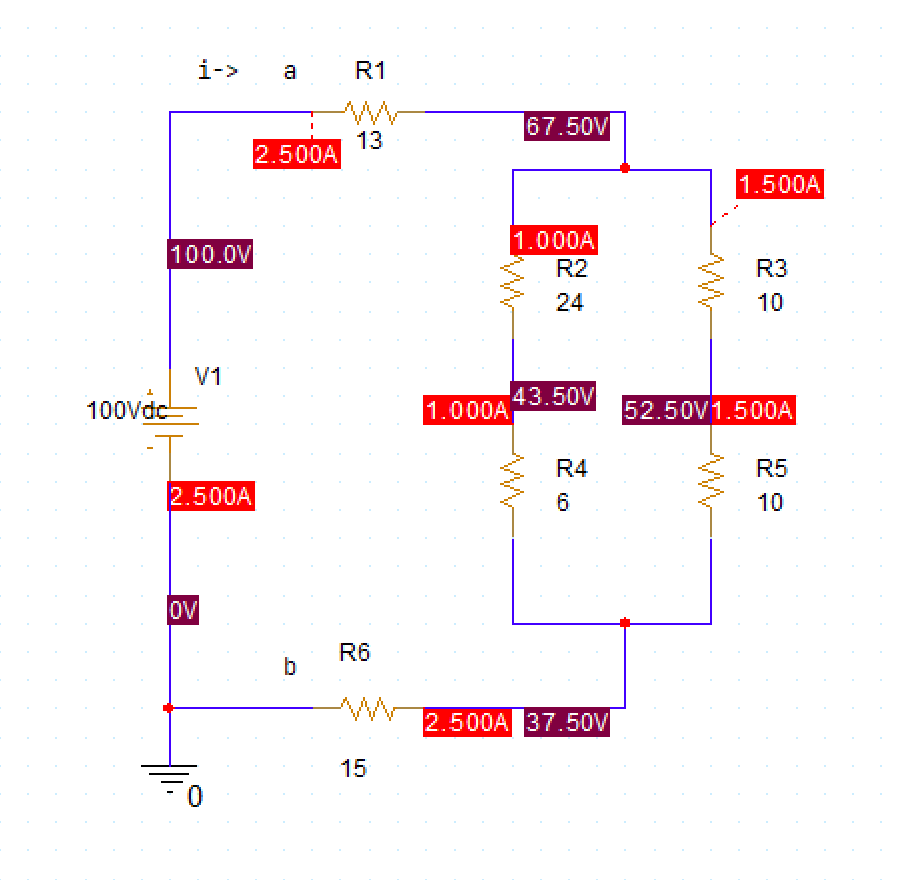
\includegraphics[width = 10cm]{source/picture/bai_1/ex6_sim.png}
\end{figure}
\newpage

\subsection{Exercise 7}
Given the following circuit. Apply the knowledge you've learned to transform it into another form in which you can find total equivalent resistance more easily. Next, find the value of the current $I_S$ through the circuit and perform a simulation to check it out.

\begin{figure}[H]
    \centering
    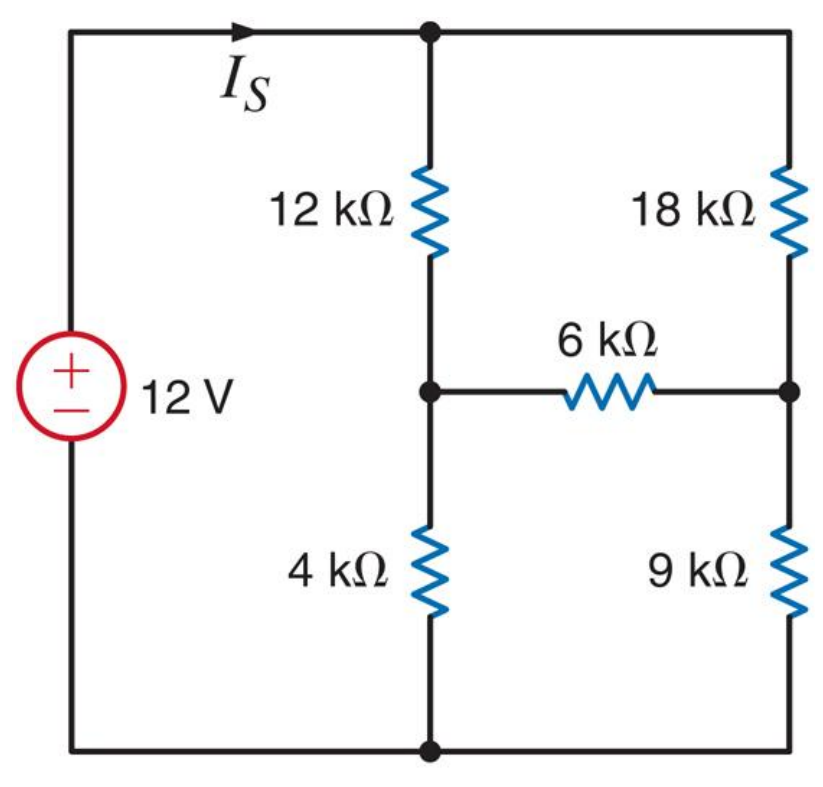
\includegraphics[width = 6cm]{source/picture/bai_1/lab1_ex7_de.png}
    \caption{Transform the circuit, then find the equivalent resistance and the current $I_S$ through the circuit.}
    \label{lab1_ex7_de}
\end{figure}

\subsubsection{Circuit transformation}
\textit{Insert the transformed circuit here.}
\begin{figure}[H]
    \centering
    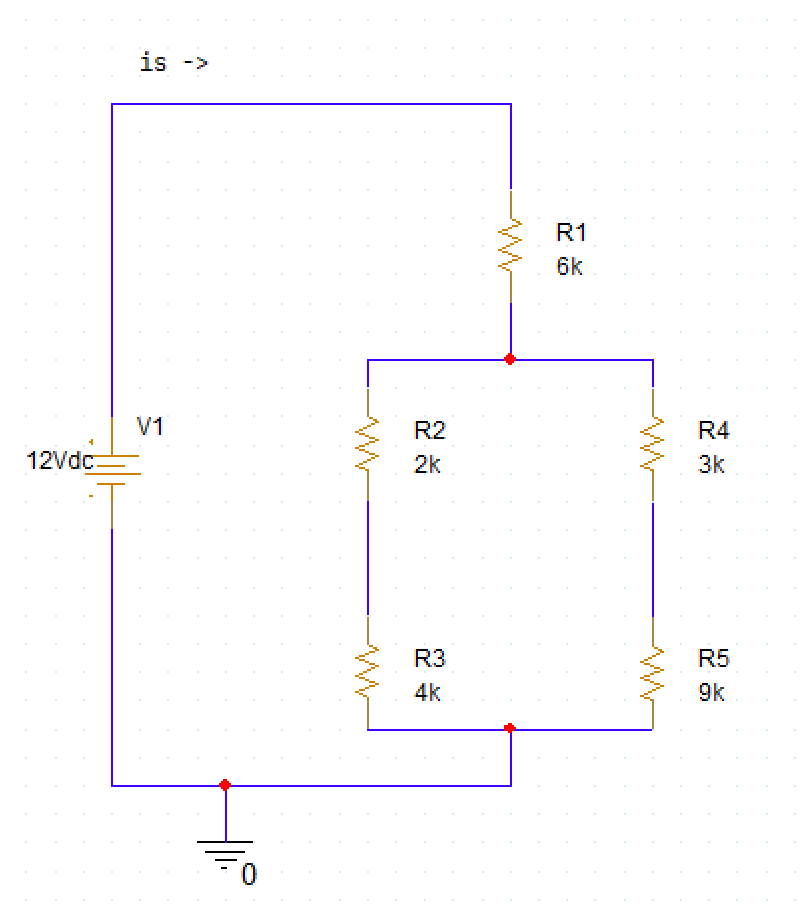
\includegraphics[width = 10cm]{source/picture/bai_1/ex7_rearrange.png}
\end{figure}
\newpage
\textit{Explain any calculations (i.e., write out the formulas you used).}\\
\bigskip
Apply Delta - Wye transformation formular:
$$ R_1 = \frac{R_aR_b}{R_a + R_b + R_c} = \frac{12\cdot 18}{12 + 18 + 6} = 6 (k\Omega)$$
$$ R_2 = \frac{R_bR_c}{R_a + R_b + R_c} = \frac{12\cdot 6}{12 + 18 + 6} = 2 (k\Omega)$$
$$ R_4 = \frac{R_aR_c}{R_a + R_b + R_c} = \frac{6\cdot 18}{12 + 18 + 6} = 3(k\Omega)$$
\bigskip



\subsubsection{Calculation}
\textit{\textbf{Notes:}}\\
\textit{Explanations, formulas, and equations are expected rather than only results.}\bigskip\\

$R_2, R_3$ parallel with $R_4 and R_5$
$R_{equivalent} = 6 + \frac{(2+4)(3+9)}{2+4+3+9} = 10 (k\Omega)$\dotfill\bigskip\\
$I_S = \frac{V_1}{R_{eq}} = \frac{12}{10\times10^{3}} = 1.2 mA$\dotfill\bigskip

\subsubsection{Simulation}
\textit{\textbf{Simulation result (image):}}
\begin{figure}[H]
    \centering
    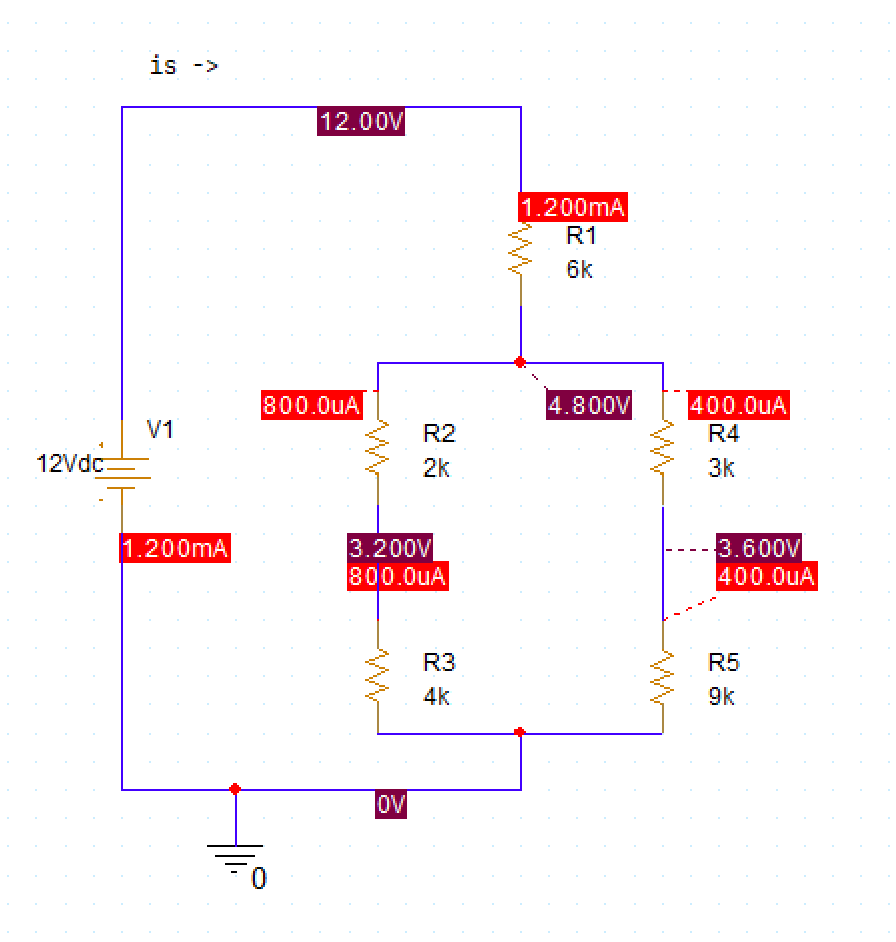
\includegraphics[width = 10cm]{source/picture/bai_1/ex7_sim.png}
\end{figure}
\newpage

\subsection{Exercise 8}
Given the following circuit with $p_2$, $p_3$, and $p_4$ are absorbing powers of unknown electrical elements. First, use the knowledge you've learned to identify whether they are active or passive elements (supplying or absorbing power). To an element absorbing power, use a pure resistor with a proper value as a representative. To a power element, use an ideal DC voltage source with the corresponding value as a representative. Next, redraw the circuit and calculate the power that each element absorbs. Note that here we use the passive sign convention. Then, perform a simulation with the elements determined by the previous step.

\begin{figure}[H]
    \centering
    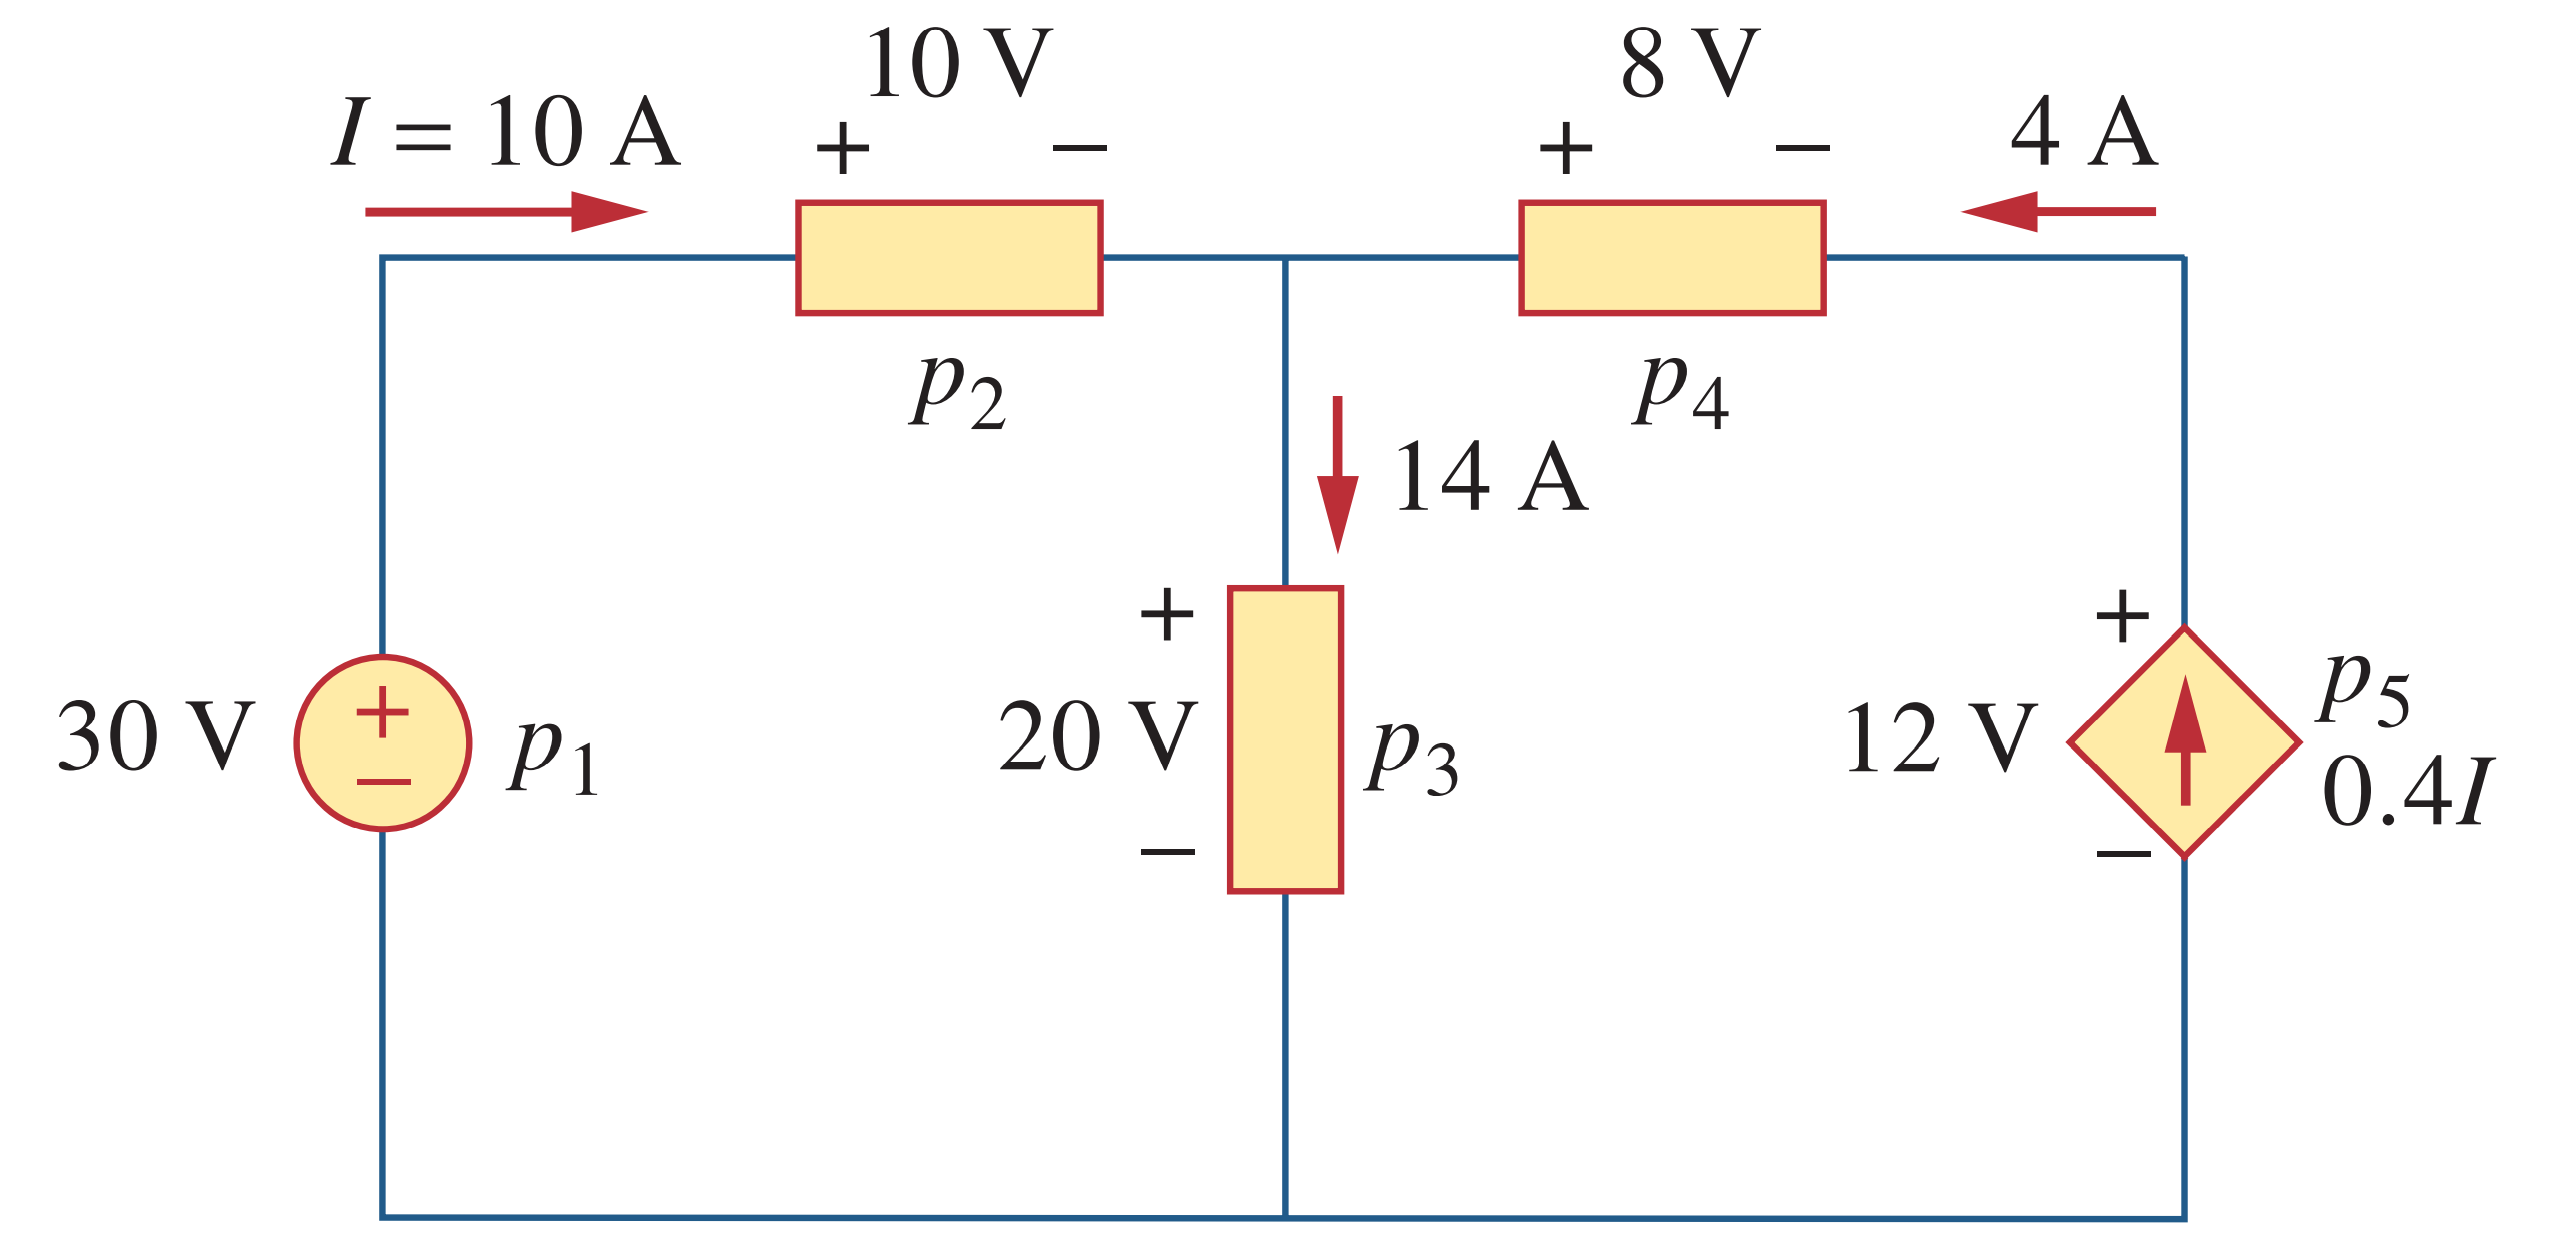
\includegraphics[width =  10cm]{source/picture/bai_1/lab1_ex8_de.png}
    \caption{Determine the unknown elements and calculate the absorbing power of each}
    \label{lab1_ex8_de}
\end{figure}

\subsubsection{Identify the unknown elements}
In Figure \ref{lab1_ex8_de}:\bigskip\\
$p_2 = 10 \times 10 = 100 W$  $\longrightarrow$  passive element\bigskip\\
$p_3 = 14 \times 20 = 280 W$  $\longrightarrow$ passive element\bigskip\\
$p_4 = 4 \times (-12) = -48W$  $\longrightarrow$ active element\bigskip\\

\subsubsection{Redraw the circuit for simulation}
\textit{\textbf{Simulation result (image):}}
\begin{figure}[H]
    \centering
    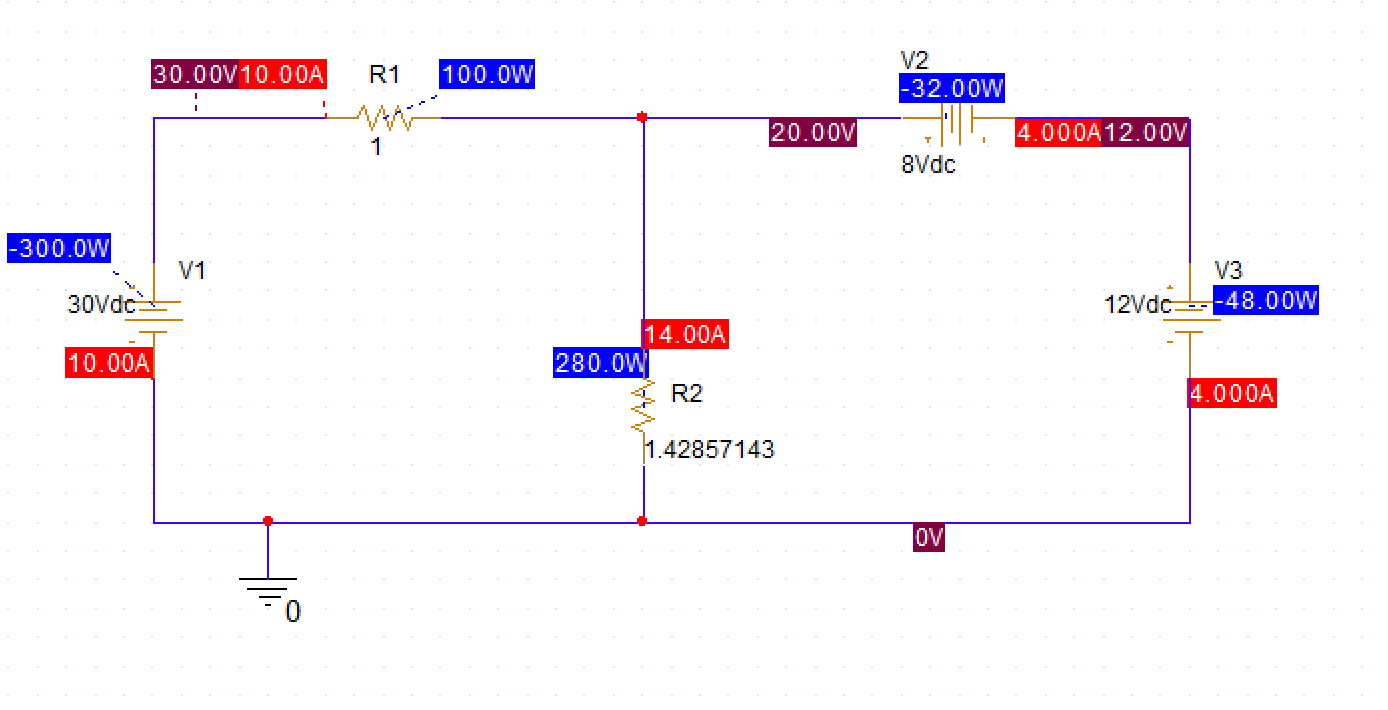
\includegraphics[width = 10cm]{source/picture/bai_1/ex8_sim.png}
    \label{ex8_rearrange}
\end{figure}
\newpage

\subsection{Exercise 9}
Given the following circuit. Find the voltage $v$ and the current $i_x$. According to the result, determine the elements whose absorbing power respectively $p_1$ and $p_2$ are active or passive (calculations are required). Note that here we use the passive sign convention. If an element consumes power, use a pure resistor with an appropriate value as a representative. If it is a  power supply element, use a corresponding ideal DC voltage source to represent it. Perform a simulation to check how the circuit works.

\begin{figure}[H]
    \centering
    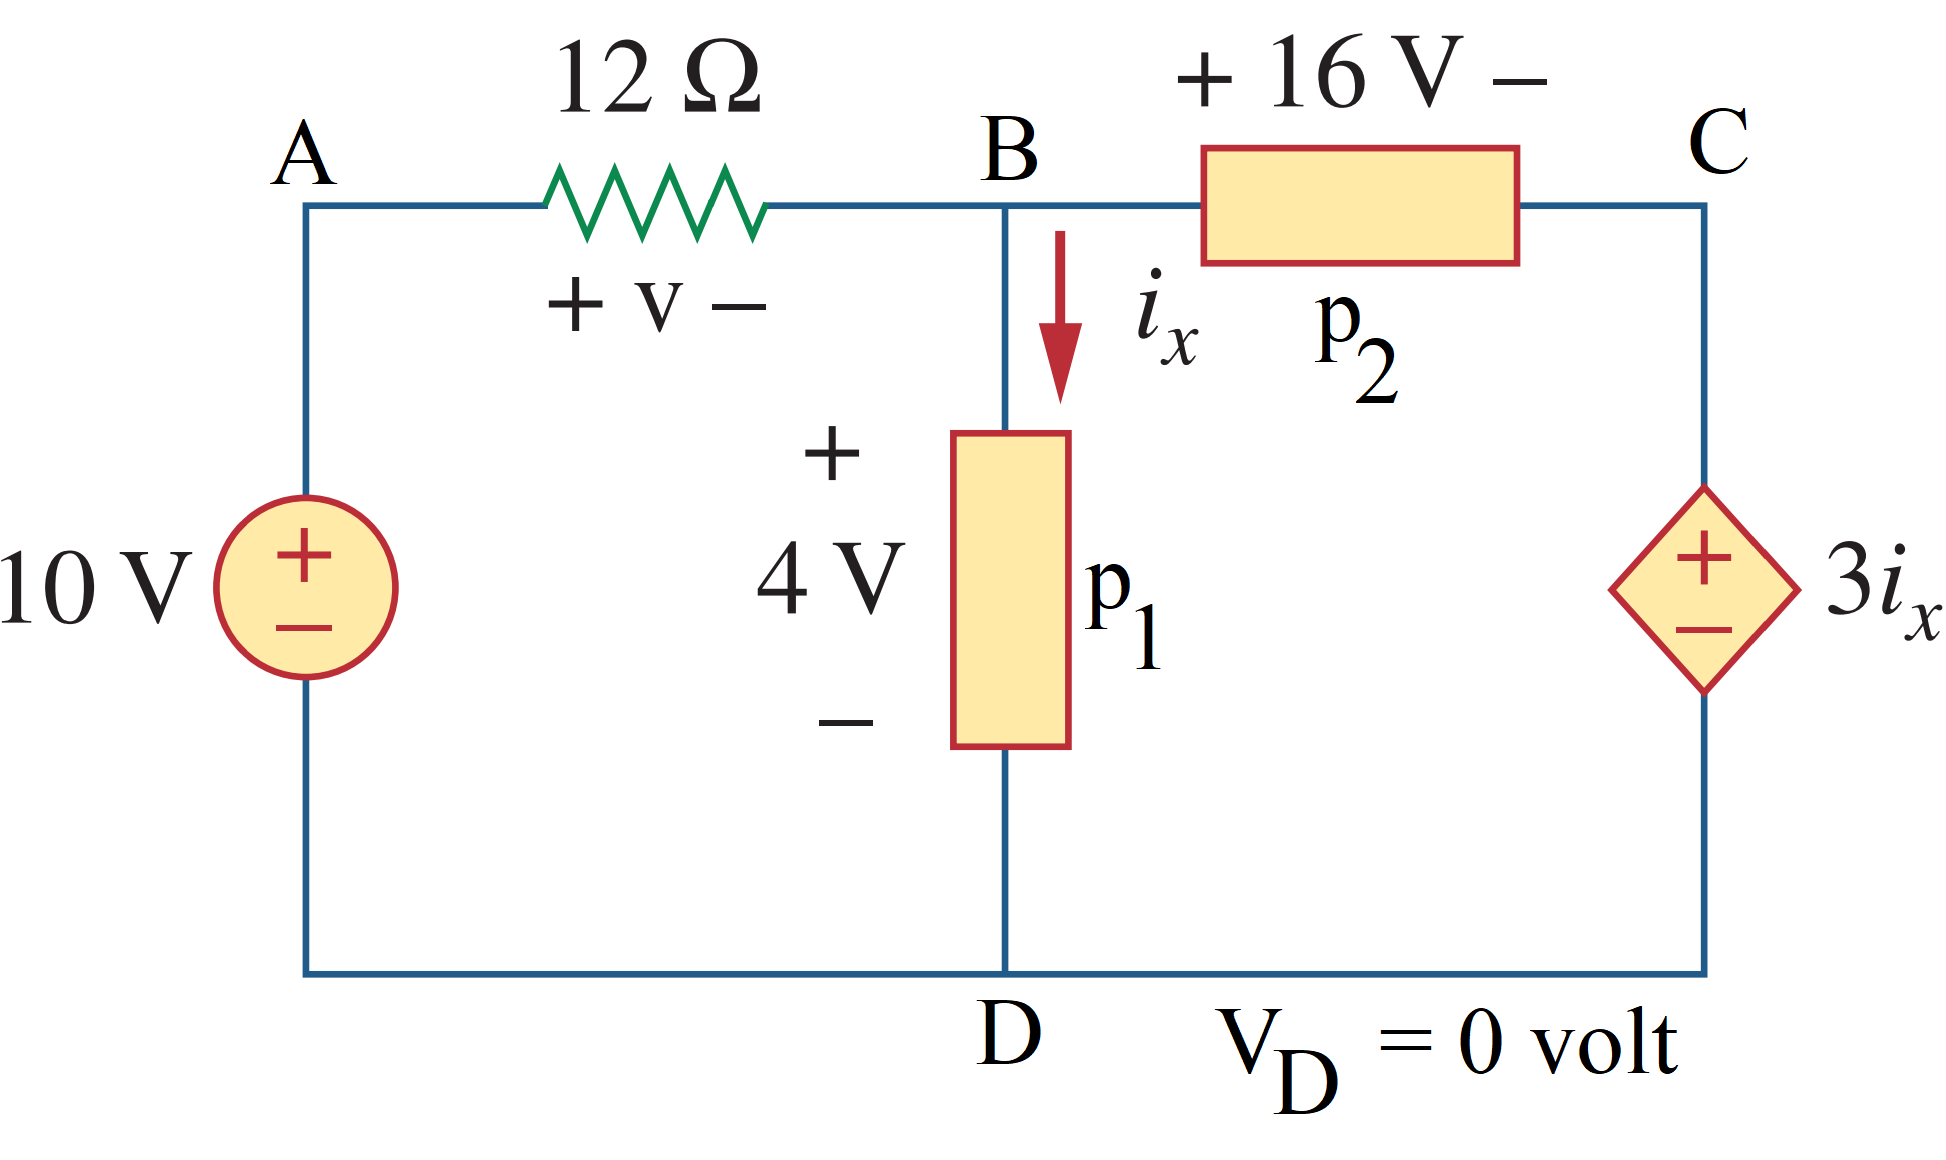
\includegraphics[width=8cm]{source/picture/bai_1/lab1_ex9_de.png}
    \caption{Find the unknown elements and variables, then check them out by simulation}
    \label{lab1_ex9_de}
\end{figure}

\subsubsection{Calculation}
\textit{\textbf{Notes:}}\\
\textit{Explanations, formulas, and equations are expected rather than only results.}\\

According to the: Kirchoff's Voltage Law \dotfill\bigskip\\
We have:\bigskip\\
$10 - v  - 4 = 0 \Rightarrow v = 6V$\dotfill\bigskip\\
$3i_x + 16 - 4  = 0 \Rightarrow i_x = -4 A$\dotfill\bigskip\\
So, we have:\bigskip\\
$p_1 = -4 \times 4 = -16$\dotfill $\longrightarrow$ active element.\bigskip\\
$I_{AB} = \frac{v}{12} = 0.5A$ \dotfill\bigskip\\
$I_{BC} = I_{AB} - i_x = 0.5 - (-4) = 4.5A$ \dotfill\bigskip\\
$p_2 = 4.5 \times 16 = 72(W)$\dotfill $\longrightarrow$  passive element.\bigskip\\
$U_{CD} = 3i_x = 3 \cdot (-4) = -12(V)$\dotfill\bigskip\

\subsubsection{Simulation}

\textbf{\textit{Tips:}}\\
To get the Current Controlled Voltage Source (CCVS) from the PSpice, under the \textit{\textbf{Place}} menu, find \textbf{\textit{PSpice Component > Source > Controlled Sources > CCVS}}.\\

A circuit used for the simulation in this exercise maybe like this:
\begin{figure}[H]
    \centering
    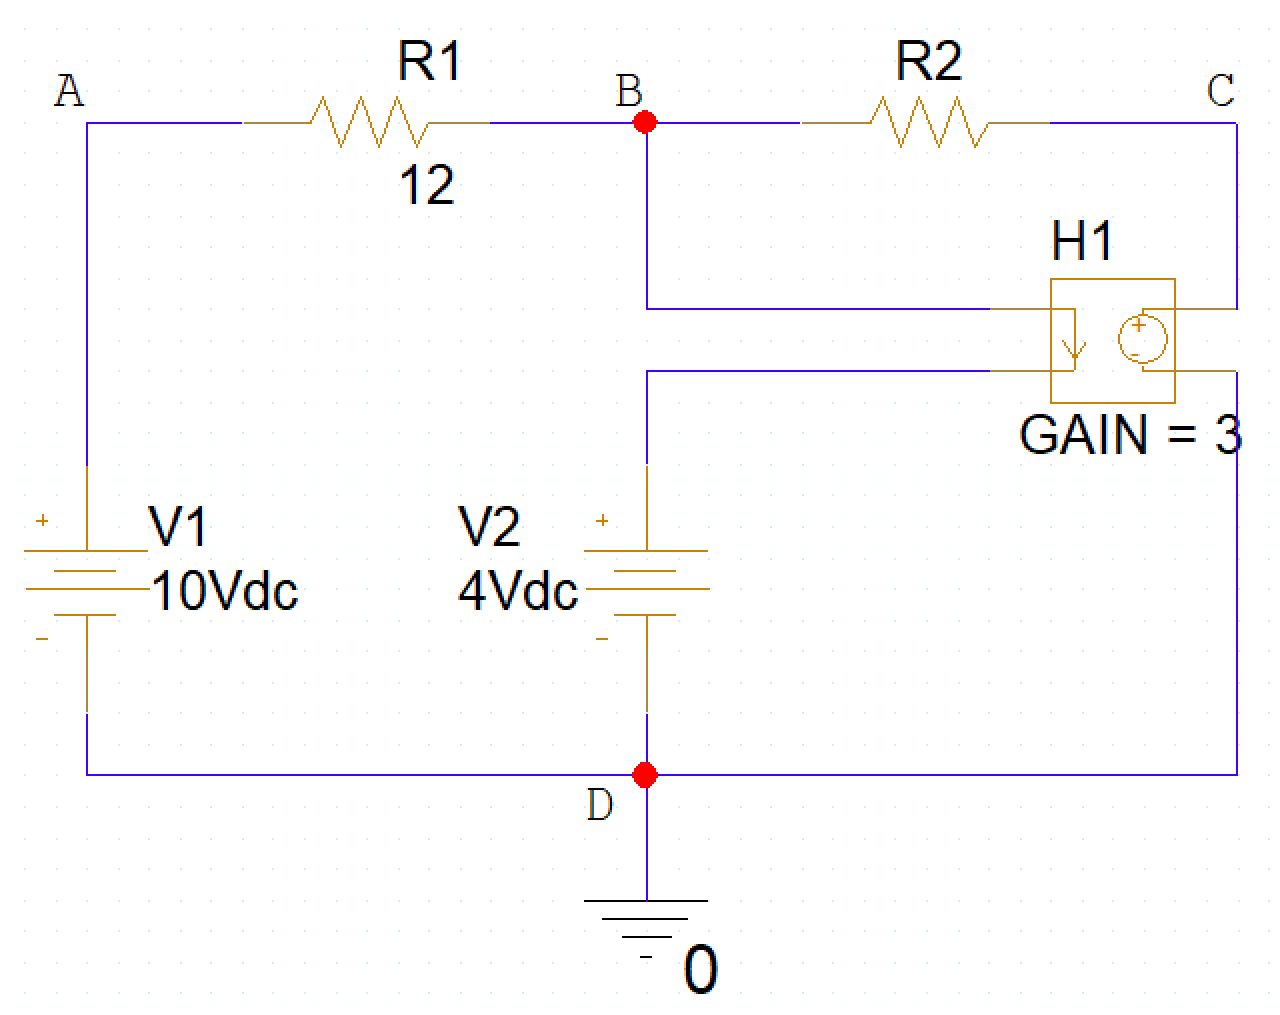
\includegraphics[width = 10cm]{source/picture/bai_1/lab1_ex9_ps.png}
    \caption{A circuit containing a Current Controlled Voltage Source in PSpice}
    \label{lab1_ex9_ps}
\end{figure}

\textit{\textbf{Simulation result (image):}}
\begin{figure}[H]
    \centering
    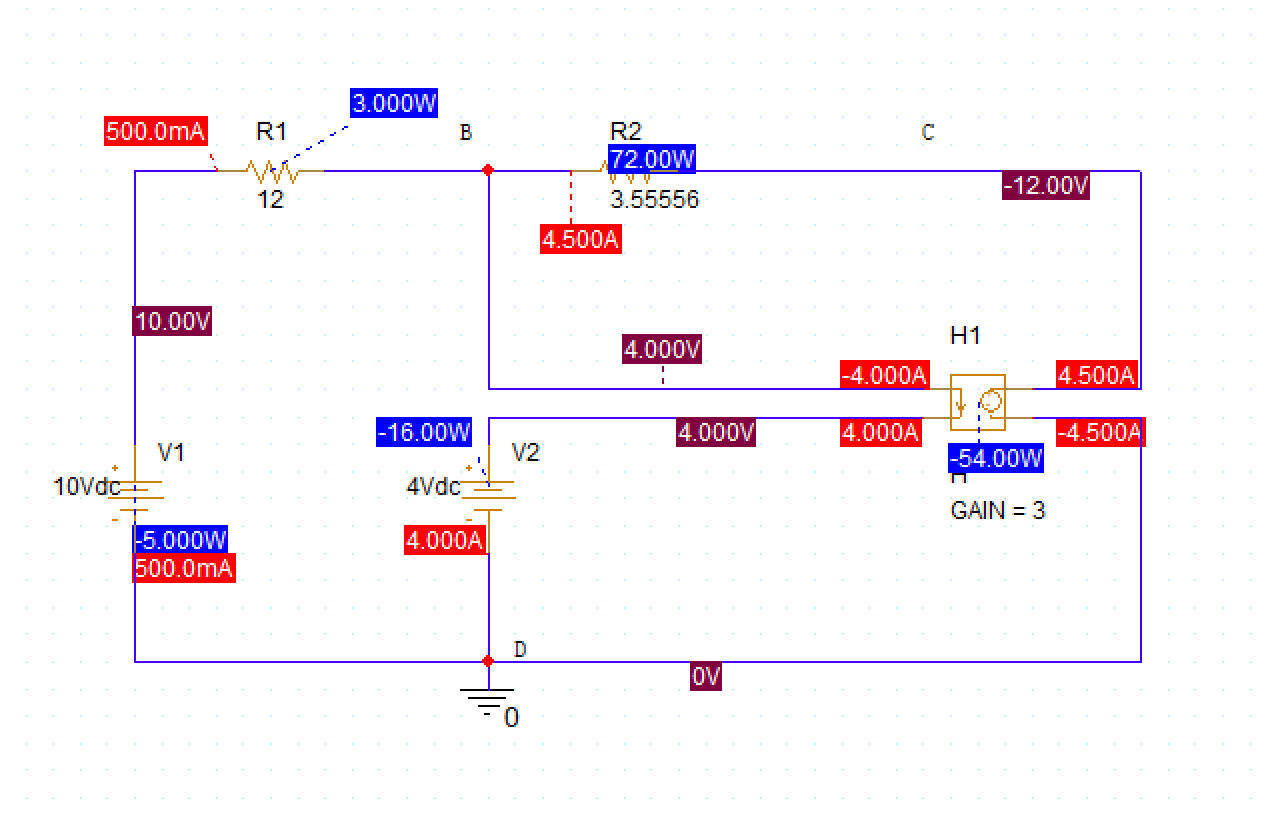
\includegraphics[width = 10cm]{source/picture/bai_1/ex9_sim.png}
\end{figure}
\newpage

\subsection{Exercise 10}
Given the following circuit. Find the voltage V. You can do this in any way but remember to explain it in detail. Then simulate the circuit to check the result.

\begin{figure}[H]
    \centering
    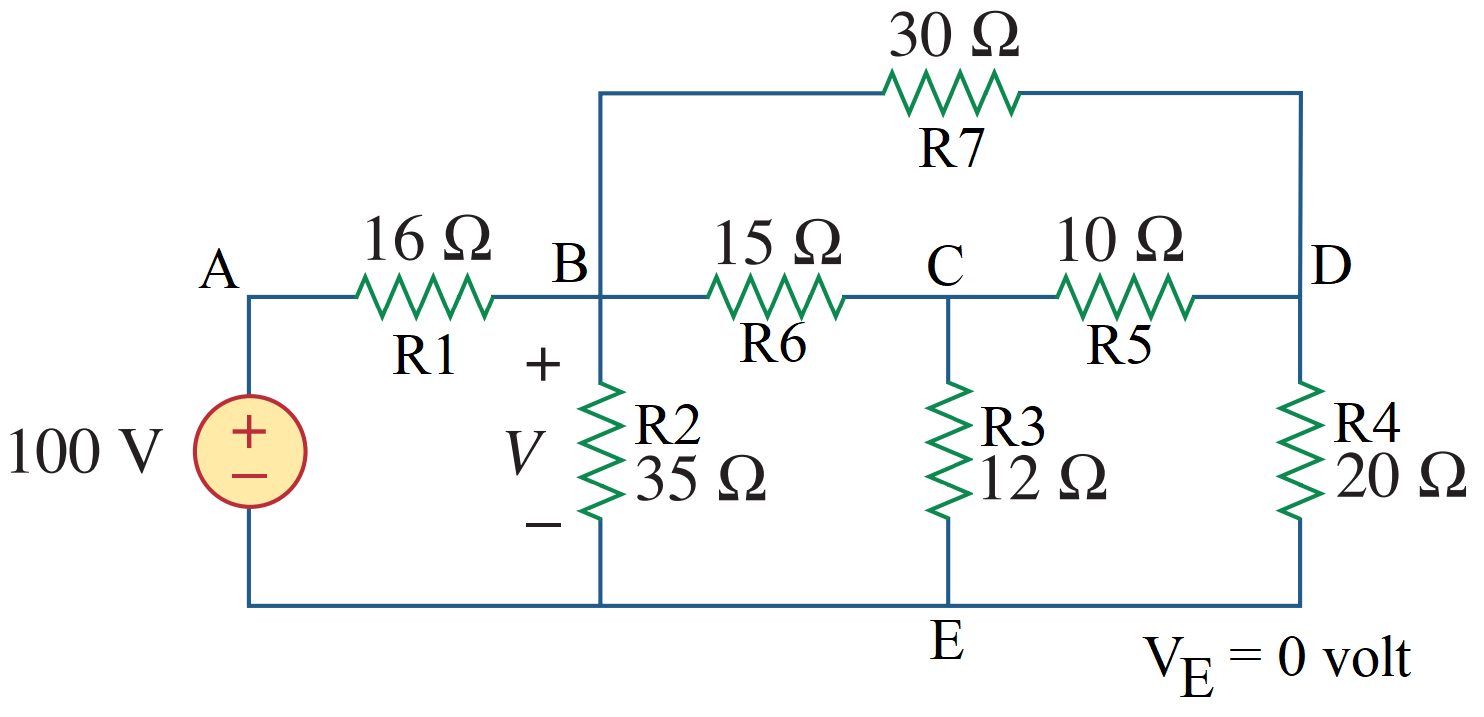
\includegraphics[width=9cm]{source/picture/bai_1/lab1_ex10_de.png}
    \caption{Find the voltage V}
    \label{lab1_ex10_de}
\end{figure}
Answer:
\begin{figure}[H]
    \centering
    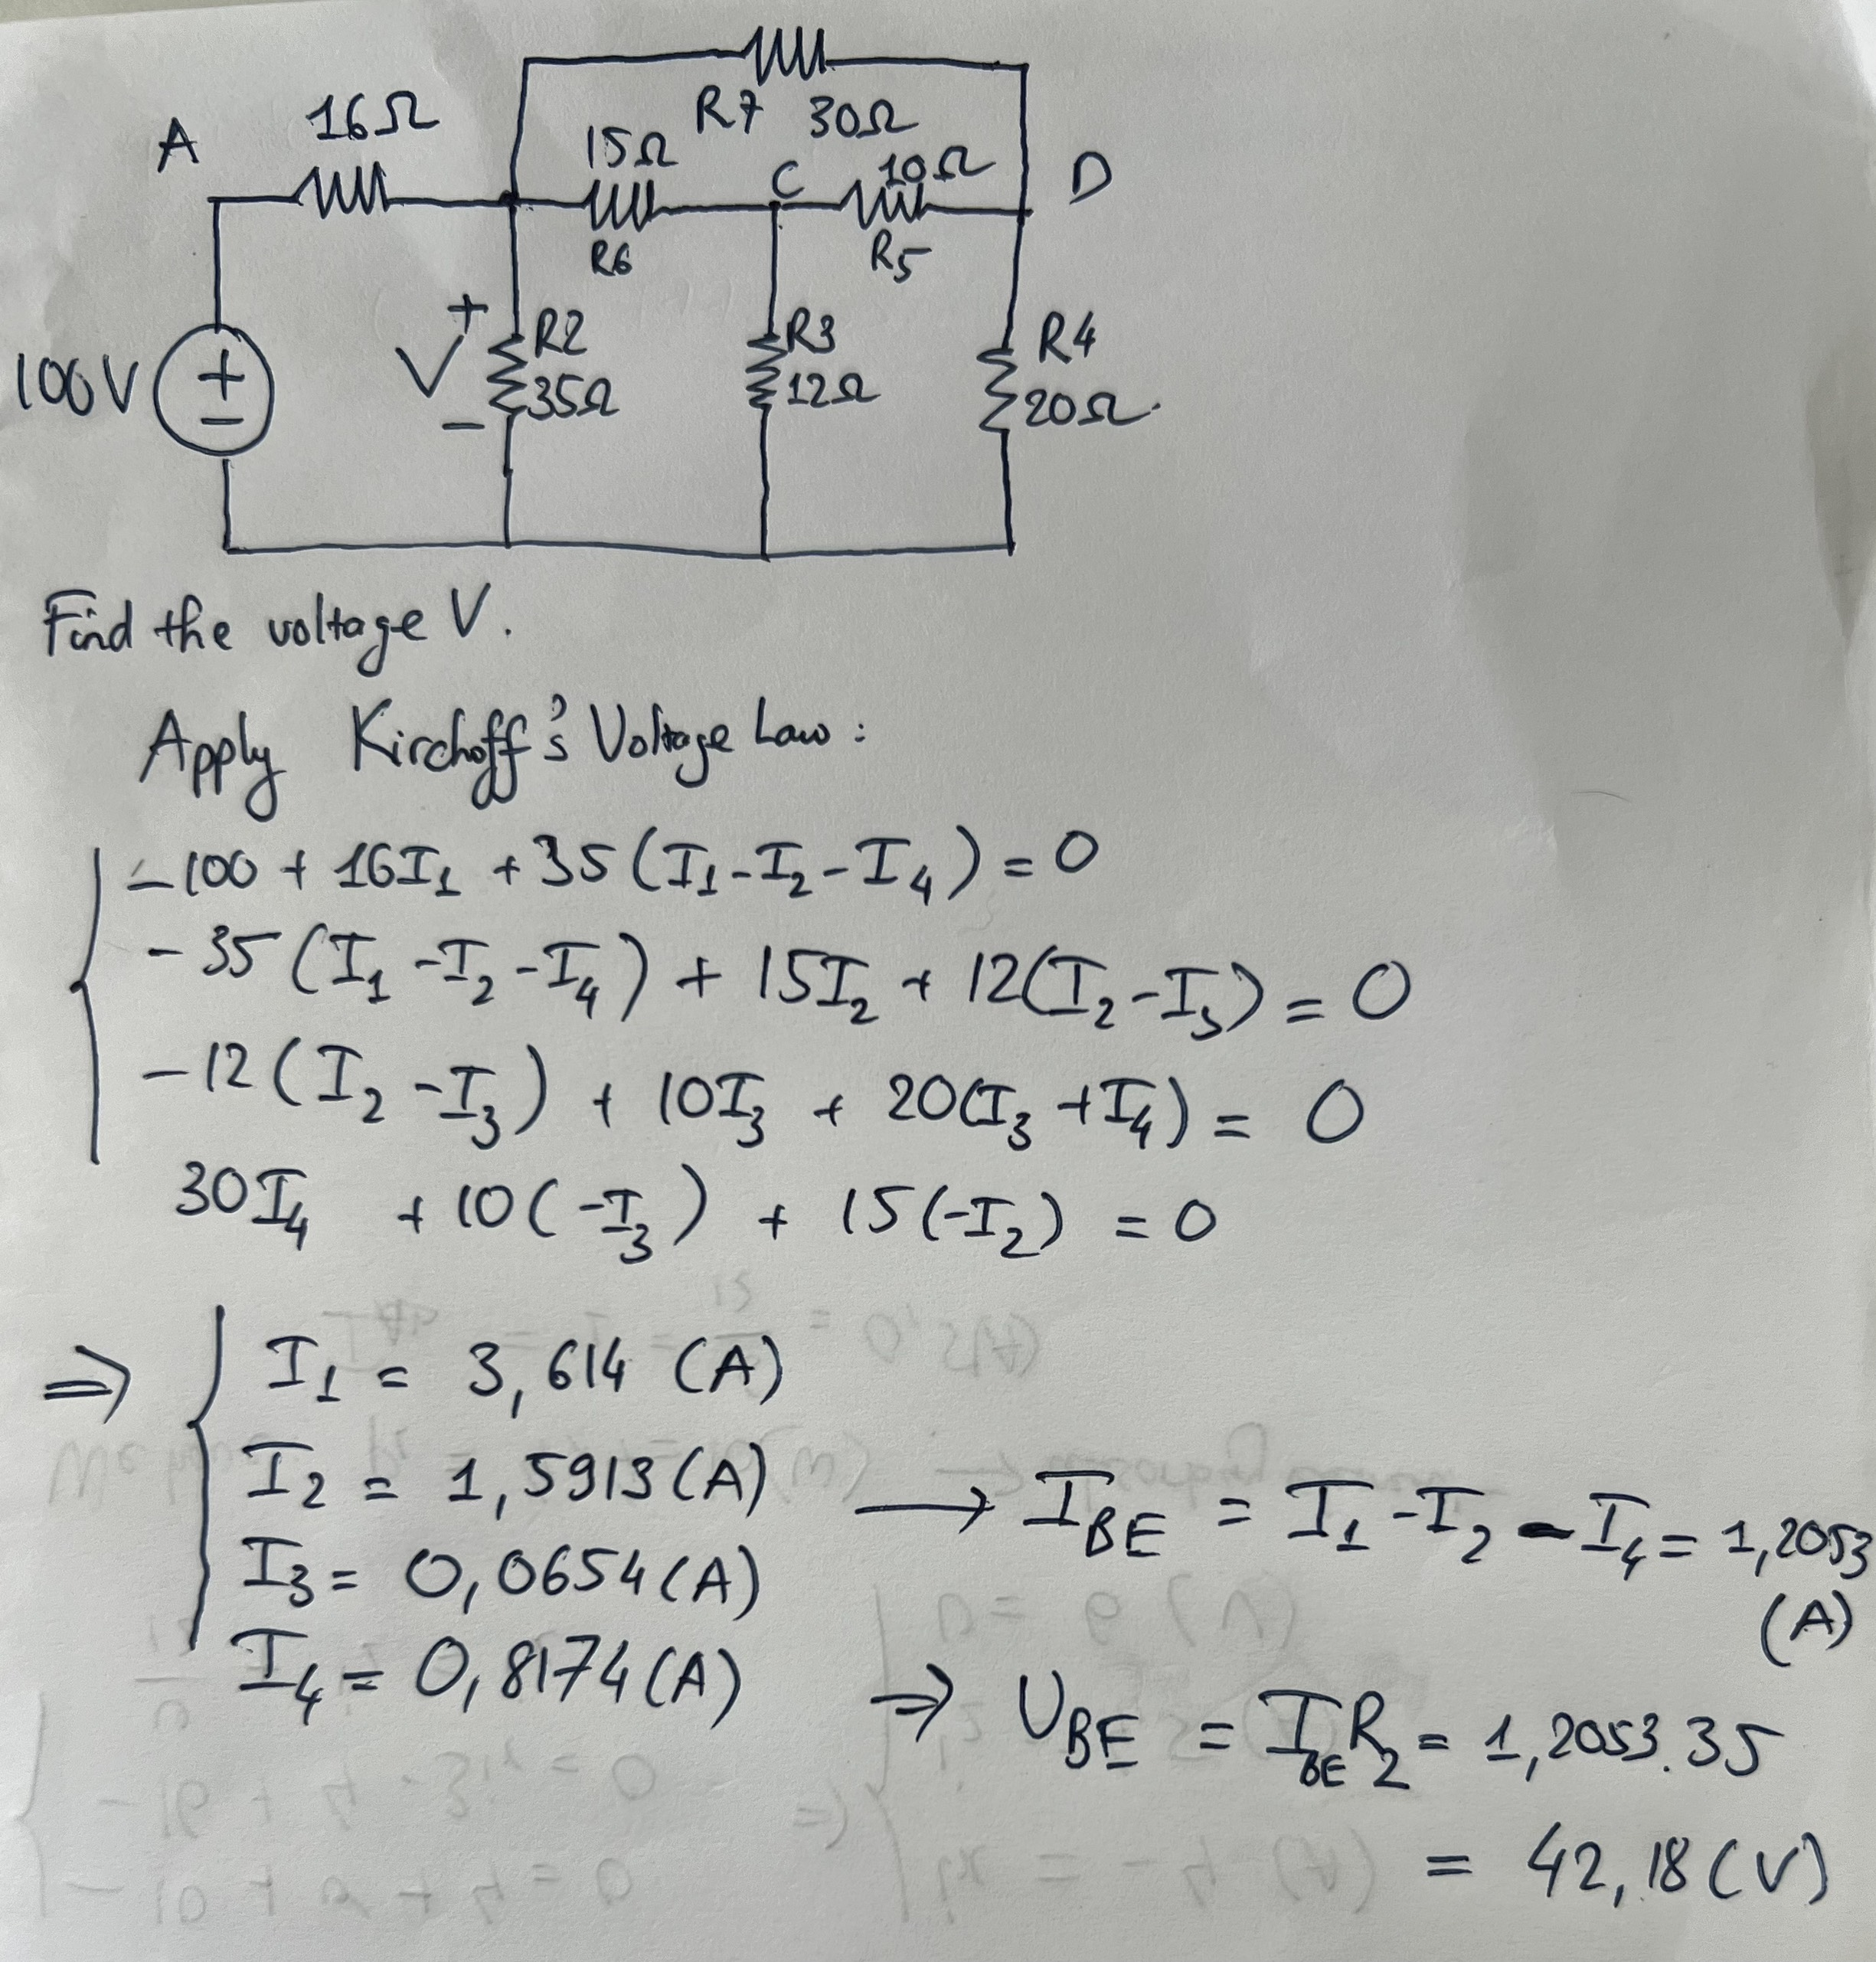
\includegraphics[width=9cm]{source/picture/bai_1/ex10_calculation.jpg}
\end{figure}

\bigskip\\
\textit{\textbf{Simulation result (image):}}
\begin{figure}[H]
    \centering
    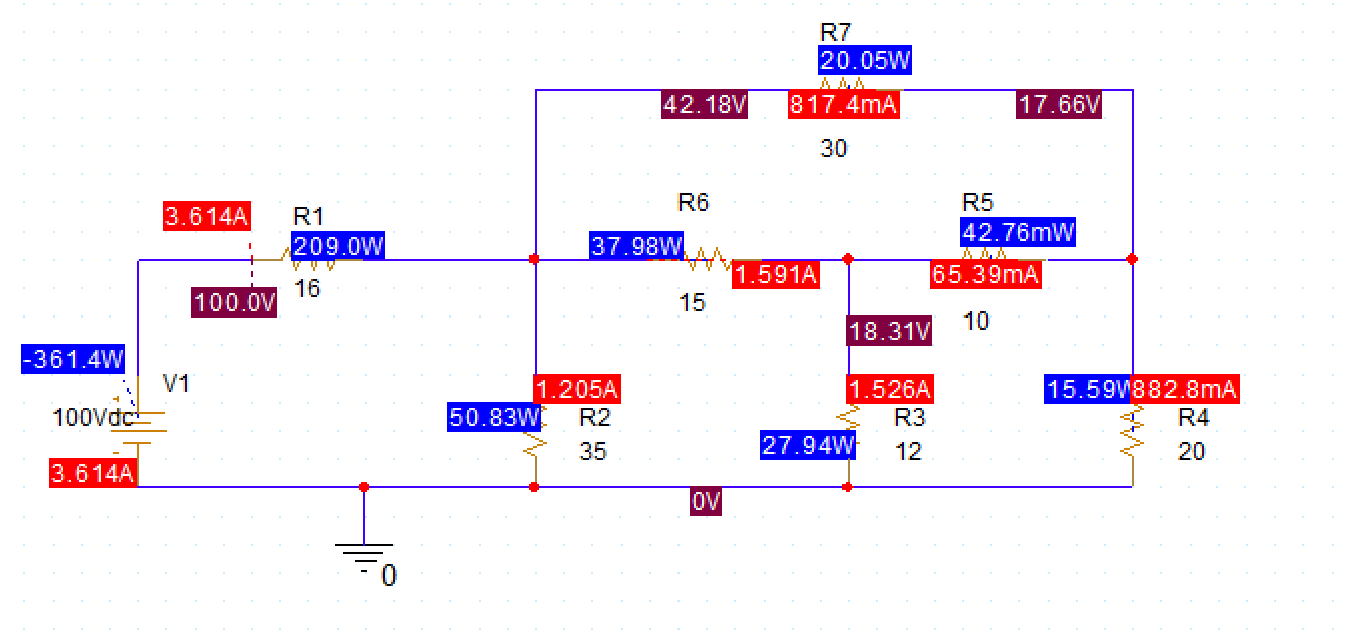
\includegraphics[width = 10cm]{source/picture/bai_1/ex10_sim.png}
\end{figure}



% \dotfill\medskip\par\mbox{}\dotfill

% \if\answer1
%   Provide the solution here
% \else
%   The solution is hide
% \fi \\